\documentclass[10pt,letterpaper,singlecolumn]{article}
\usepackage{setspace}
\doublespacing
\usepackage{latex8}
\usepackage{times}
\usepackage{cite}
\usepackage{subfigure}
\usepackage{psfig}
\usepackage[pdftex]{graphicx}
\usepackage{epsfig}
\usepackage{pstricks}
\usepackage{fullpage}
\usepackage{amsthm}
\usepackage{graphics}
\usepackage{comment}
\usepackage[small,compact]{titlesec}
\usepackage[small,it]{caption}
\usepackage{wrapfig}
\usepackage{enumerate}
\usepackage{multirow}

\begin{document}

\title{CSE530 Project Final Report\\
Bandwidth-Aware Memory Hierarchy Design with Hybrid Memory Technologies}

\author{Cong Xu and Jishen Zhao\\
\{czx102, juz138\}@psu.edu\vspace{-10pt}
}
\maketitle

\begin{large}

\begin{abstract}
  \boldmath Chip-multiprocessor~(CMP) is a promising solution for high
  performance computing systems. However, the limited increases in main memory
  bandwidth results in a growing bandwidth gap between the processor cores and
  the main memory, which becomes a potential obstacles to system performance
  improvement. In this project, we explore bandwidth-aware memory hierarchy
  design with various emerging memory technologies. Based on the observations
  obtained from our pre-exploration of various emerging memory technologies, we
  evaluate systerm performance obtained with various cache hierarchy
  configurations. With different applications, we evaluate the optimal shared
  cache configurations in a CMP system, in terms of the number of shared cache
  levels, memory technology and capacity of each level. We show that cache
  hierarchy with hybrid memory technologies benefits system performance with
  non-write-intensive applications.

\end{abstract}

% ------------------------------------------------------------------------------

\section{Introduction}

Many of modern chip-multiprocessors are designed to perform well on various
applications to achieve high performance by exploiting their inherent
parallelism. Such systems support large number of threads and single instruction
multiple data~(SIMD) execution, which puts a lot of pressure on the memory
system. Typically, memory latency is not a bottleneck, since the latency can be
hidden via multi-threading or hardware prefetching. To this end, bandwidth
becomes a potential bottleneck. A high rate of computing often brings in a high
rate of data transitions. In some cases, the working set of an application fits
in the on-die caches, which can typically provide sufficient bandwidth to keep
up with the processing cores. However, if the working set does not fit in the
on-die caches, the main memory needs to provide much of the data. Since the
bandwidth of off-chip main memory is quite limited, applications with such
working sets are potentially bandwidth-bound. Therefore, it is crucial to design
the memory hierarchy to overcome the bandwidth limitation.

It is known that performance improvement of a computing system can be achieved
via multiple memory levels. Adding an extra level of memory, however, can also
help alleviate the bandwidth bottleneck of off-chip memory. Specifically, we
would like to examine (1) the number of levels in the optimal memory hierarchy,
(2) the appropriate memory technology of each level, and (3) the capacity and
bandwidth of each level. We will also explore the energy-efficiency of the
memory hierarchy design constrain, and the memory hierarchy design within a
fixed power budge.\vspace{0.15in}

% -----------------------------------------------------------------------------
\section{Motivation}

Throughput computing involves performing a huge number of calculations with a large amount of parallelism. Throughput computing applications span many domains and are already critical on a variety of platforms from high-performance computing (HPC) machines to commercial servers to client machines.

Systems designed to perform well on throughput computing applications achieve high performance by exploiting their inherent parallelism. These systems support large numbers of threads and/or use wide SIMD execution. This puts a lot of pressure on the memory system. Fortunately, memory latency is typically not a bottleneck since the latency can be hidden via multithreading or hardware prefetching, since the data access patterns are relatively simple. On the other hand, bandwidth is a potential bottleneck.

Many throughput computing applications have inherently large working sets (i.e., tens to hundreds of MB). These are unlikely to fit in conventional on-die SRAM caches for the foreseeable future. Further, unlike more traditional workloads (e.g., those similar to SPEC or TPC benchmarks), many throughput computing applications see a sharp drop in performance once caches are too small to hold their working sets. Thus, these applications are likely to be bandwidth-bound at main memory unless some significant changes are made to the memory hierarchy.

Unfortunately, there are few simple techniques to improve bandwidth efficiency of a system. While there is some work in this area~\cite{BW-Wall}, this is insufficient for the large bandwidth requirements of some throughput computing applications. So today��s systems that tout good performance for throughput computing applications (e.g., nVidia��s Tesla) do so by providing large main memory bandwidths via the use of GDDR rather than improving bandwidth efficiency. However, GDDR has fairly strict capacity limits and is much more power hungry than conventional DRAM modules. This reduces its desirability for throughput computing, and makes it a bad choice for general purpose systems trying to improve their throughput computing performance.

Emerging memory technologies such as Magnetoresistive Random Access Memory~(MRAM), Phase-Change Memory~(PCM), Resistive Random Access Memory~(RRAM),
embedded DRAM, have shown potential to to be used as on-chip caches and the main memory~\cite{Sun:2009:MRAM-L2-CMP}. Therefore, we explore how to enhance the memory hierarchy from the bandwidth point of view.


% -----------------------------------------------------------------------------

\section{Emerging Memory Technologies}

We first review the technology background three types of non-volatile memories, which are STT-RAM, PCRAM, and RRAM.

\subsection{STT-RAM}
STT-RAM uses the magnetic property of the material and uses Magnetic Tunnel Junction (MTJ) as its binary storage.  As shown in Fig.~\ref{fig:mram_cell}, MTJ contains two ferromagnetic layers and one tunnel barrier layer. The direction of one ferromagnetic layer is fixed, which is called the reference layer, while the direction of the other one can be changed by passing a driving current, which is called the free layer. The relative magnetization direction of two ferromagnetic layers determines the resistance of MTJ.  If two ferromagnetic layers have the same directions, the resistance of MTJ is low, indicating a ``0" state; if two layers have different directions, the resistance of MTJ is high, indicating a ``1" state.

\begin{figure*}[htbp]
% The "!" means to maintain the aspect ratio.
\centering
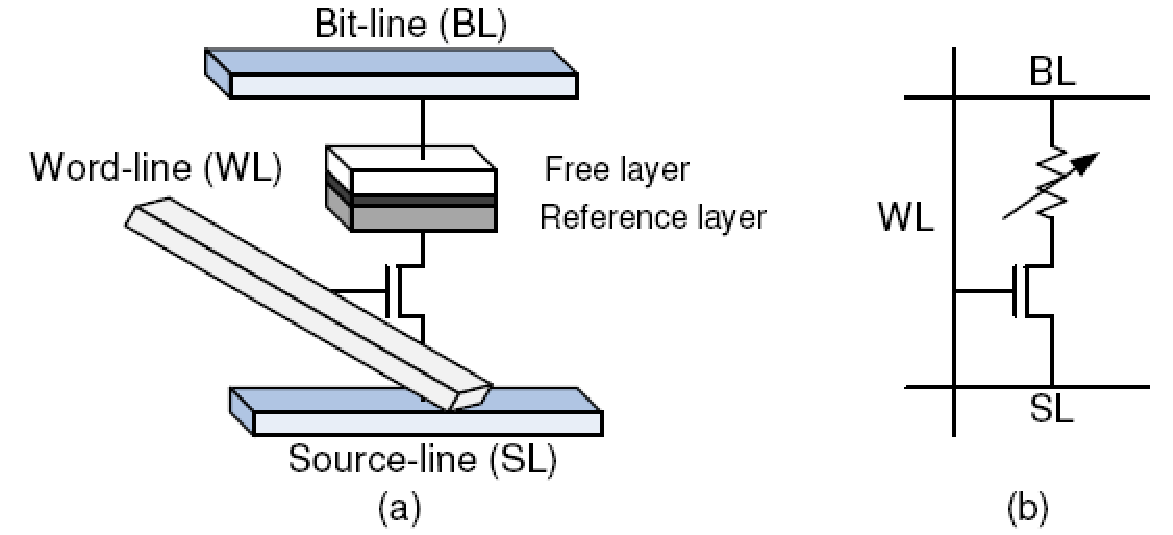
\includegraphics[width=3in]{figures/mram_cell}
\caption{Demonstration of a MRAM cell. (a) Structural view. (b) Schematic view.}
\label{fig:mram_cell}
\end{figure*}

\subsection{PCRAM}

PCRAM uses chalcogenide-based material to storage informations.  The chalcogenide-based materials in recent PCRAM research are usually alloys of germanium, antimony, and tellurium (GeSbTe, or GST), which can be switched between a crystalline phase (SET or ``1" state) and an amorphous phase (RESET or ``0" state) with the application of heat. The crystalline phase shows high optical reflectivity and low electrical resistivity, while the amorphous phase is characterized by low reflectivity and high resistivity.

\begin{figure*}[htbp]
% The "!" means to maintain the aspect ratio.
\centering
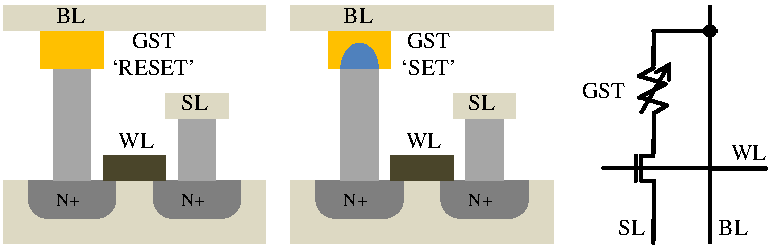
\includegraphics[width=3in]{figures/GST}
\caption{The schematic view of a PCRAM cell with MOSFET selector transistor (BL=Bitline, WL=Wordline, SL=Sourceline}
\label{fig:GST}
\end{figure*}

\subsection{RRAM}

\begin{figure*}[htbp]
% The "!" means to maintain the aspect ratio.
\centering
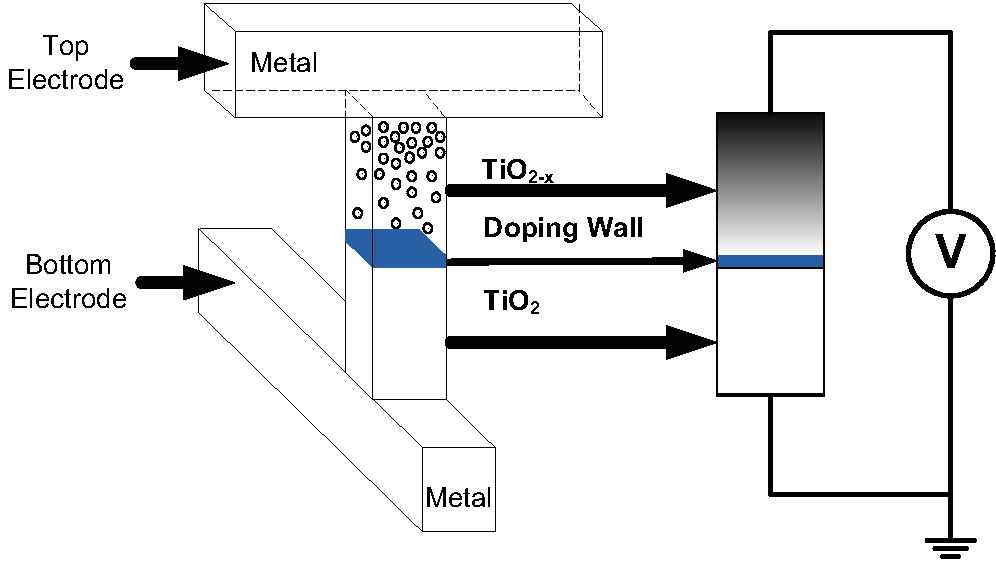
\includegraphics[width=3in]{figures/memristor}
\caption{The conceptual view of the structure of memristor cells.}
\label{fig:memristor}
\end{figure*}

Memristor, a portmanteau of ``memory resistor'', is a generalized resistance that maintains a functional relationship between the time integrals of current and voltage.  Memristor was first theoretically predicted by Chua in 1971~\cite{memristor:chua} as the fourth fundamental circuit element from the completeness of relations between the four basic circuit variables, namely, current, voltage, charge, and flux-linkage.  The first memristor practical demonstration was presented by Williams \emph{et al.} in 2008~\cite{memristor:missing}.  Fig.~\ref{fig:memristor} shows a conceptual view of the memristor structure~\cite{memristor:missing}. The top electrode and bottom electrode are two metal nanowires on platinum, and the thin titanium dioxide film is sandwiched by the electrodes.

% -----------------------------------------------------------------------------
\section{Memory Technology Pre-Exploration}
Many modeling tools have been developed during the last decade to enable system-level design exploration for SRAM- or DRAM-based cache and memory design.  For example, CACTI~\cite{CACTI} is a tool that has been widely used in the computer architecture community to estimate the speed, power, and area of SRAM and DRAM caches. In addition, CACTI has also been extended to evaluate the performance, power, and area for STT-RAM~\cite{CACTI:DAC08:Dong}, PCRAM~\cite{CACTI:GLSVLSI08:Mangalagiri,CACTI:PCRAMsim}, and NAND flash~\cite{CACTI:DATE10:Mohan}. However, as CACTI is originally designed to model SRAM-based cache, some of its fundamental assumptions do not match the actual NVM circuit implementation, and thereby these CACTI-like estimation tools do not model the NVM array organization in the exact way that the chip is fabricated. In this section, we use \emph{NVSim}, a circuit-level model for NVM performance, energy, and area estimation, which supports various NVM technologies including STT-RAM, PCRAM, RRAM, and conventional NAND flash.

\begin{figure*}[htbp]
% The "!" means to maintain the aspect ratio.
\centering
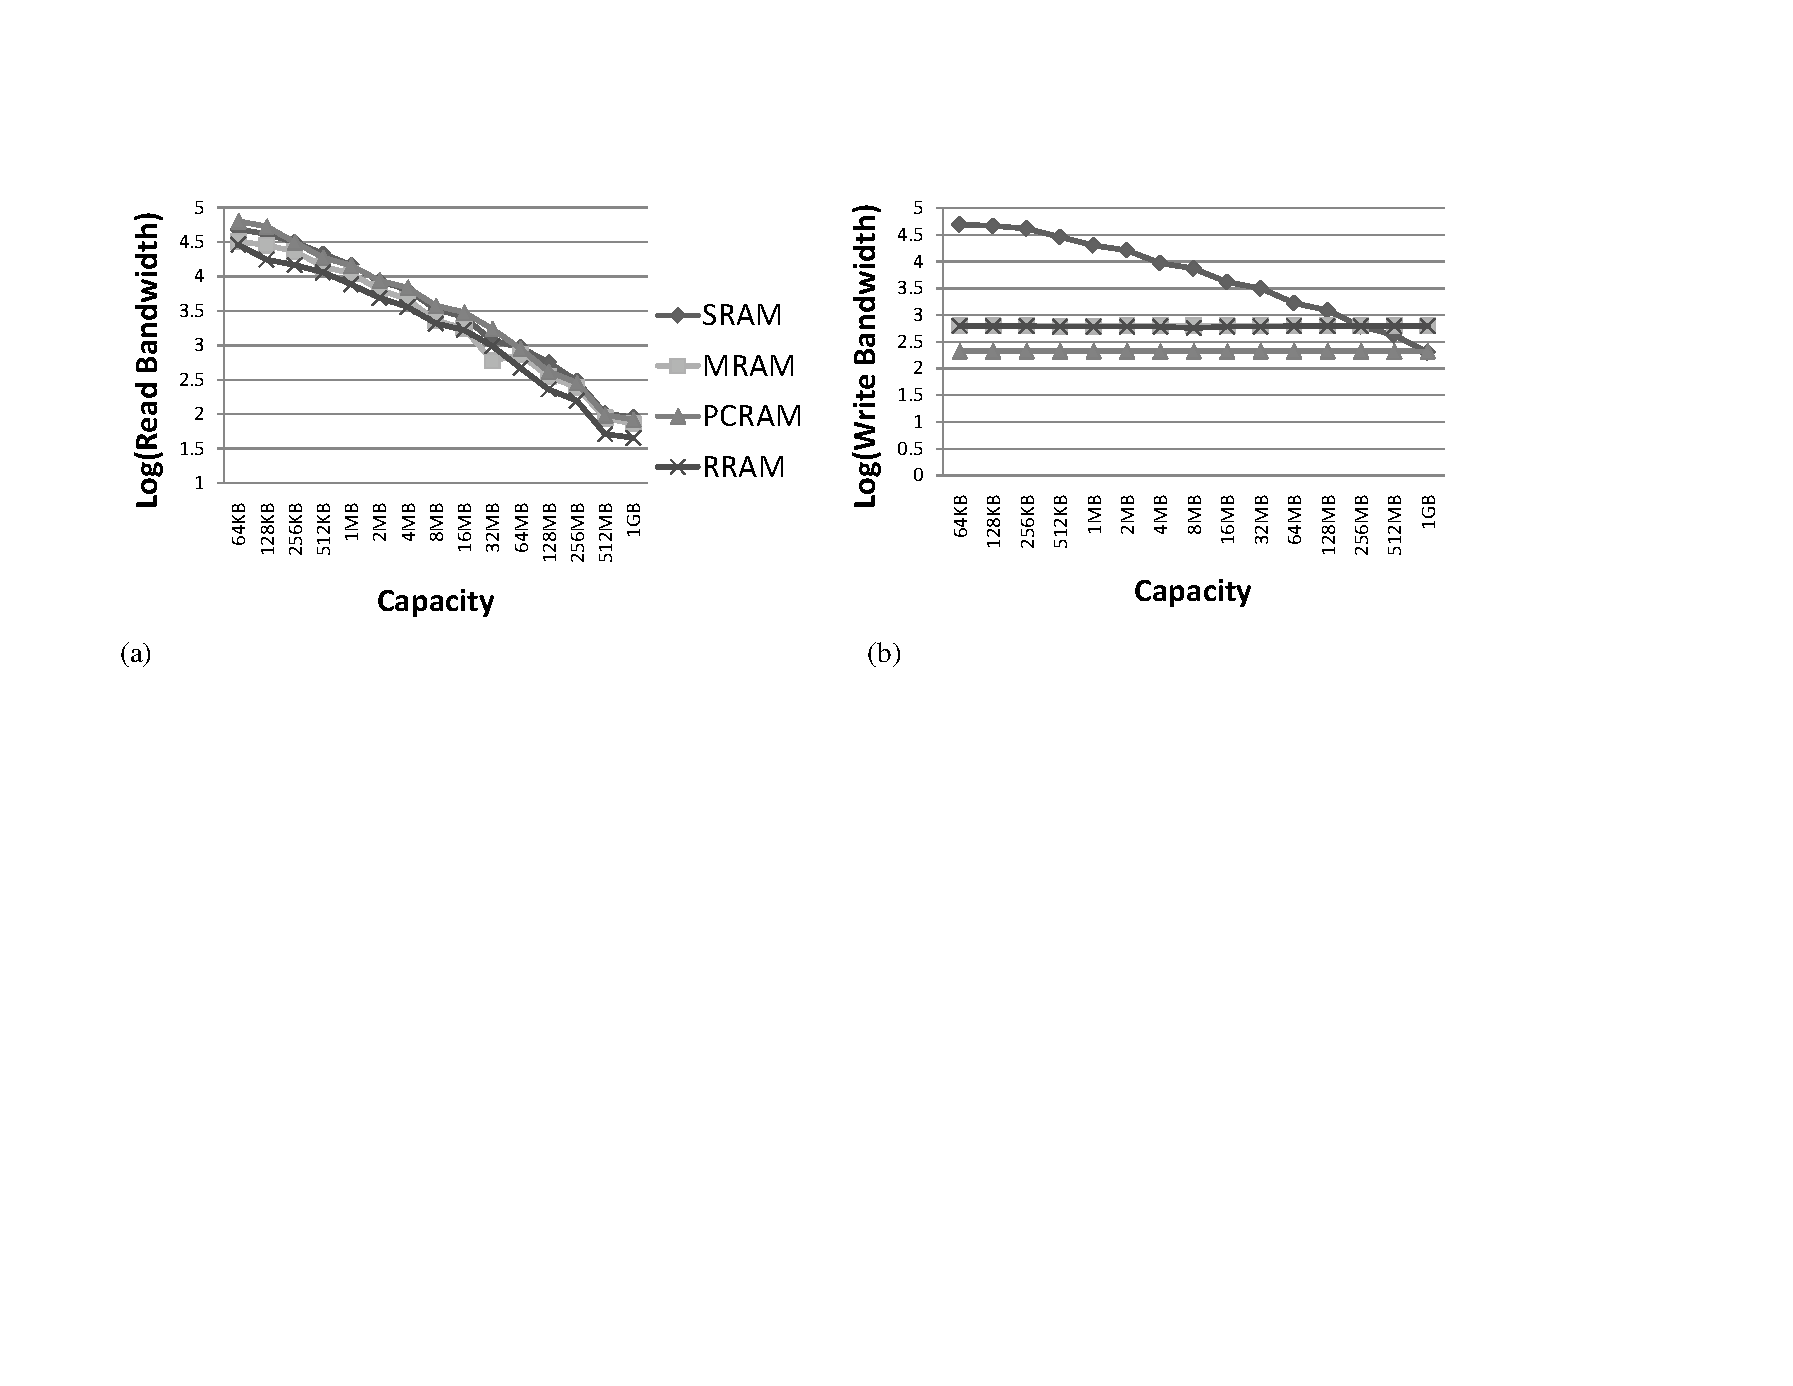
\includegraphics[width=6in]{figures/RAM_bandwidth}
\caption{Read and write bandwidths provided by different memory technologies.
(a) Read bandwidth provided by different memory technologes. (b) Write bandwidth
provided by different memory technologies.}
\label{fig:memory-bw}
\end{figure*}

First of all, we estimate the read and write bandwidths that can be provided by different memory technologies. Figure~\ref{fig:memory-bw} shows the results, with both x- and y-values in \emph{log} scale. The figure illustrates both the
provided read and write bandwidth as a function of memory capacity. Each of the memory technologies actually provide nearly the same read bandwidths, as is shown in figure~\ref{fig:memory-bw}(a). On the other hand, a straight forward observation from figure~\ref{fig:memory-bw}(b) is that the write bandwidth varies among different memory technologies. The shape of the SRAM write bandwidth curve is very similar to the read bandwidth curve. The write bandwidth curves of the other three memory technologies appear to be very different. The reason is that write latencies of the three non-volatile memories are much higher than read latencies. Another observation from figure~\ref{fig:memory-bw}(b) is that the curves cross to each other at different locations.

\begin{figure*}[htbp]
% The "!" means to maintain the aspect ratio.
\centering
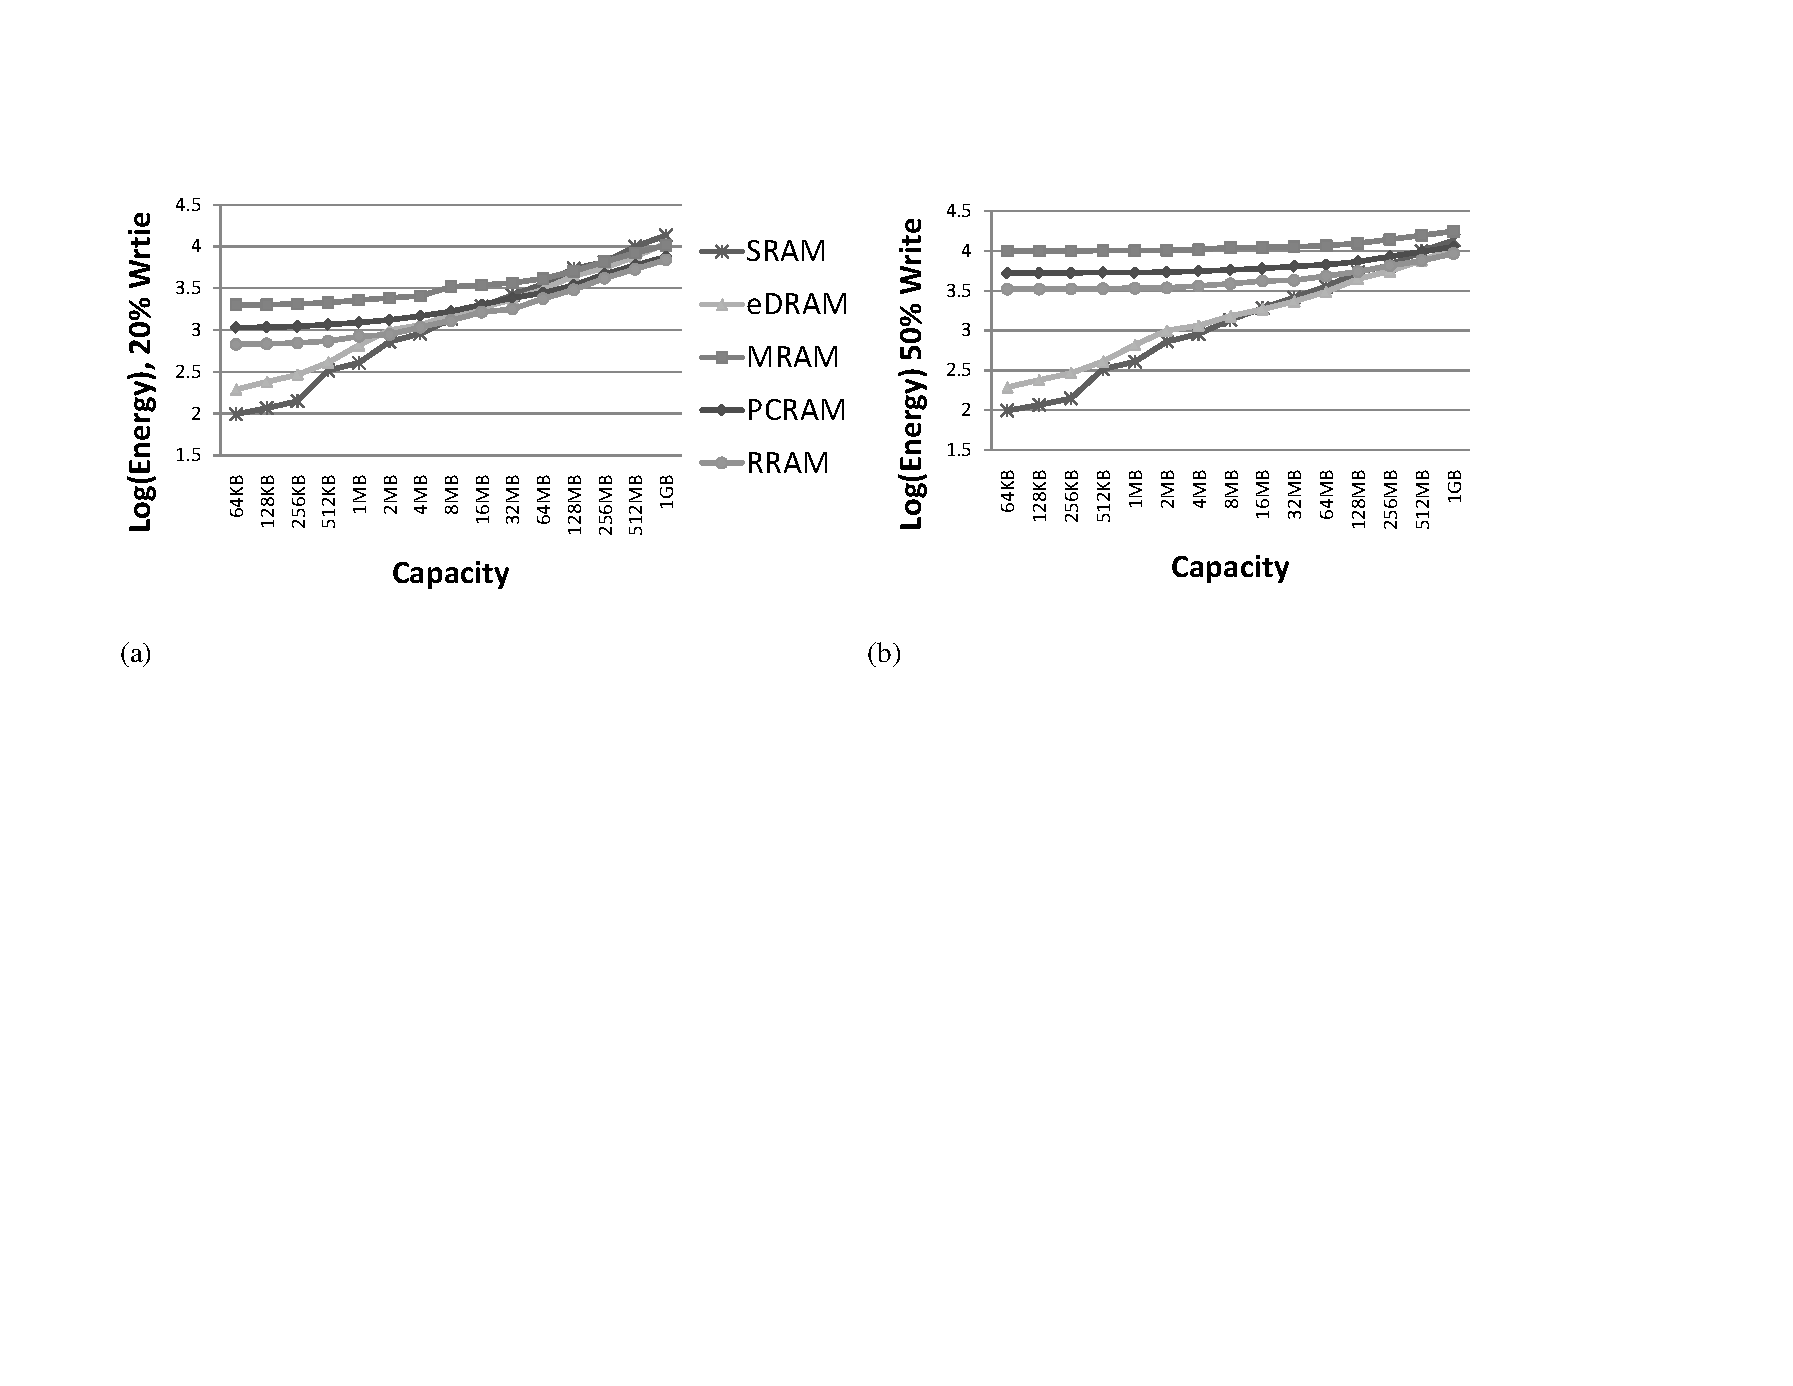
\includegraphics[width=6in]{figures/RAM_energy}
\caption{Dynamic energy consumption with the provided bandwidths of different
  memory technologies. (a) Dynamic Energy with 20\% write.  (b) Dynamic Energy with 50\% write. }
\label{fig:memory-energy}
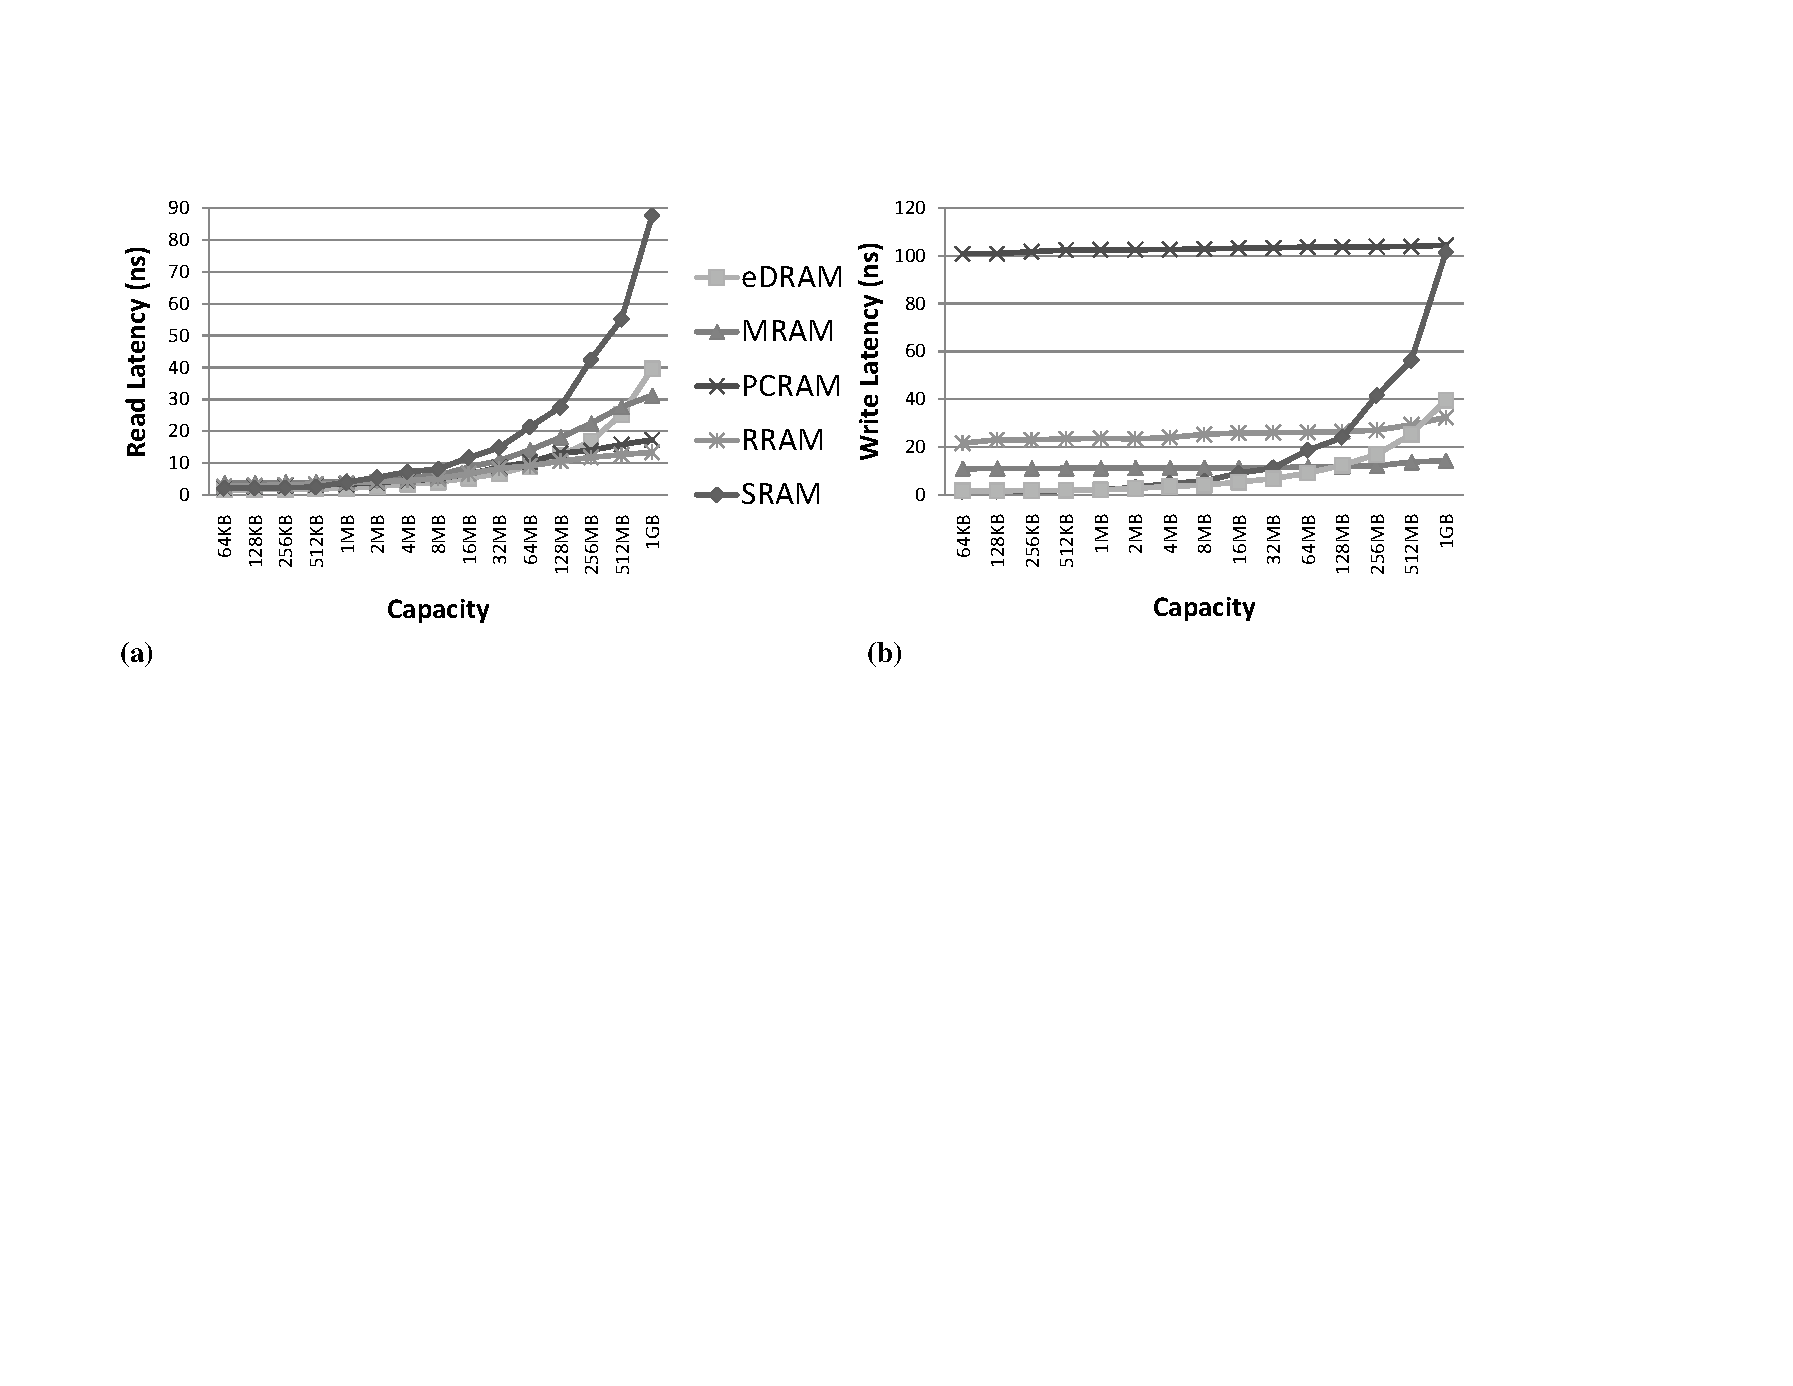
\includegraphics[width=6in]{figures/RAM_latency}
\caption{Latency of different memory technologies. (a) Read Latency. (b) Write Latency.}
\label{fig:memory-latency}
\end{figure*}

Being aware that the read and write latencies of NVM are asymmetric, we consider the read latency at first. In NVsim, we divide the entire cache read latency into the following components:
\begin{itemize}
\item (a)	H-tree input delay
\item (b)	Decoder + word-line delay
\item (c)	Bit-line delay
\item (d)	Sense Amplifier delay
\item (e)	Comparator Delay (for tag part only)
\item (f)	H-tree output delay
\end{itemize}
H-tree latency (a) and (f) are mainly determined by the RC delay of global wires, which is positive proportional to the area of memory macro. Sensing delay (d) is affected by the read noise margin of memory cell that is affected by off/on resistance ratio.


Based on these two observations, we would like to design a
bandwidth-aware hybrid memory hierarchy, which always provides the high memory
bandwidth with the given capacity. For example, we probably would like to use
1) SRAM when the memory capacity is under 256MB, 2) MRAM or RRAM between
256MB and 1GB (if only bandwidth is considered), and 3) PCRAM when the memory
cacity is over 1GB.

\section{Experiments}

Based on the parameters of different cache configurations collected from our
modified version of CACTI~\cite{CACTI}, we evaluate both pure SRAM-based and
hybrid cache hierarchy designs. In this section, we show how bandwidth-aware
memory hierarchy design method help with improving the system performance.\vspace{0.15in}

\subsection{Experimental Setup}

We use Simics~\cite{Magnusson:2002:simics-orig-paper} as the simulator in our
experiments. It is configured to model an eight-core CMP. Each core is in-order, and
is similar to UltraSPARC III architecture. The frequency of each core is set to
be 1GHz. Table~\ref{table:cmp-config} lists the detailed parameters of the
baseline. Our baseline contains 8 private L1 instruction and data caches
respectively. Since we only evaluate shared cache hierarchies, each of L1 cache
is fixed to be SRAM-based, and of 64KB capacity. As regard to lower level
caches, we evaluate two cases, pure SRAM-based and hybrid caches with various
memory technologies, including SRAM, MRAM, RRAM, and eDRAM. By evaluating both
cases, we would like to find out optimal cache design that leads to the peak
performance, i.e., the number of cache levels that is reqired, memory technology
used for each level, and capacity of each level.

\begin{table}[t]
  \centering
  \caption{Baseline CMP configuration.}
  \vspace{0.1in}
  \begin{tabular}{l|c}
    \hline
    \multicolumn{2}{l}{\textbf{Core}}\\
    \hline
    No. of cores & 8\\
    \hline
    Frequency & 1GHz\\
    \hline
    Core architecture & in-order, 14-stage pipline, 2 ALUs, 2 FPUs\\
    \hline
    \multicolumn{2}{l}{\textbf{Memory}}\\
    \hline
    \multirow{2}{*}{Private caches} & L1 I-cache: SRAM, 8 x 64KB, 64B line, 2-way, write-through \\
                                    & L1 D-cache: SRAM, 8 x 64KB, 64B line, 2-way, write-through \\
    \hline
    \multirow{2}{*}{Shared caches} & Case 1: Pure SRAM, 64B line, 8-way, write-back \\
                                   & Case 2: Hybrid~(SRAM, MRAM, RRAM, eDRAM), 64B line, 8-way, write-back\\
    \hline
    Main memory & 4GB\\
    \hline
  \end{tabular}
  \label{table:cmp-config}
\end{table}

The benchmarks are selected from PARSEC benchmark suite~\cite{PARSEC:2008} with
multithreaded programs, which focus on emerging workloads that are designed to
be representative of next-generation shared-memory programs for CMPs. Since the
performance of different memory technologies are closely related to read and
write intensities, we selected some workloads that vary in the average numbers
of L2 cache read per thousand instructions~(RPKI) and write per thousand
instructions~(WPKI), which are listed in
Table~\ref{table:benchmarks}.\vspace{0.3in}

\begin{table}[t]
  \centering
  \caption{Characteristics of selected benchmarks.}
  \vspace{0.1in}
  \begin{tabular}{l|c|c||l|c|c}
    \hline
    \textbf{Benchmarks} & \textbf{RPKI} & \textbf{WPKI} &
    \textbf{Benchmarks} & \textbf{RPKI} & \textbf{WPKI}\\
    \hline
    blackscholes & 22.8 & 61.7 & ferret & 5.7 & 173.4\\
    \hline
    bodytrack & 5.4 & 139.5 & fluidanimate & 2.6 & 70.1\\
    \hline
    canneal & 5.4 & 29.3 & streamcluster & 17.3 & 16.9\\
    \hline
    facesim & 6.0 & 102.4 & swaptions & 2.6 & 121.4\\
    \hline
  \end{tabular}
  \label{table:benchmarks}
\vspace{0.5in}
\end{table}

\subsection{Results}

We evaluate various possible configurations with shared caches by simulation,
i.e., with possible numbers of levels, memory technologies, and cache capacities
for each cache level. We consider SRAM and eDRAM as the possible memory
technologies to implement L2 and L3 caches. Both MRAM and RRAM have higher write
latency than SRAM. Furthermore, the endurance of RRAM is too low to be used as
lower level caches. Consequently, these two memory technologies are only
considered to be used as the last level cache.

In the first set of experiments, we evaluate the system performance with
two-level shared caches. Figure~\ref{fig:thput-l2l3} shows the system throughput
with all the benchmarks. It is illustrated that implementing hybrid cache with
eDRAM as the L3 cache helps with performance among most of the benchmarks. Such
performance improvement is more than 10\% in Figure~\ref{fig:thput-l2l3}(a). It
is indicated by our memory technology exploration that eDRAM shows more latency
benefits with larger capacities. As a result, a larger eDRAM-based L3 cache
leads to more performance improvement to the pure SRAM implementation, as
illustrated by Figure~\ref{fig:thput-l2l3}(b). However, hybrid cache does not
always improve the performance, as shown in Figure~\ref{fig:benchmark-l2l3}.
With the benchmark \emph{canneal}, hybrid cache configurations outperform the
pure SRAM implementation among overall range of various capacities. With the
benchmark \emph{ferret}, however, pure SRAM implementation results in higher
performance than hybrid cache implementation with the same capacity
configuration.

\begin{figure*}[t]
\centering
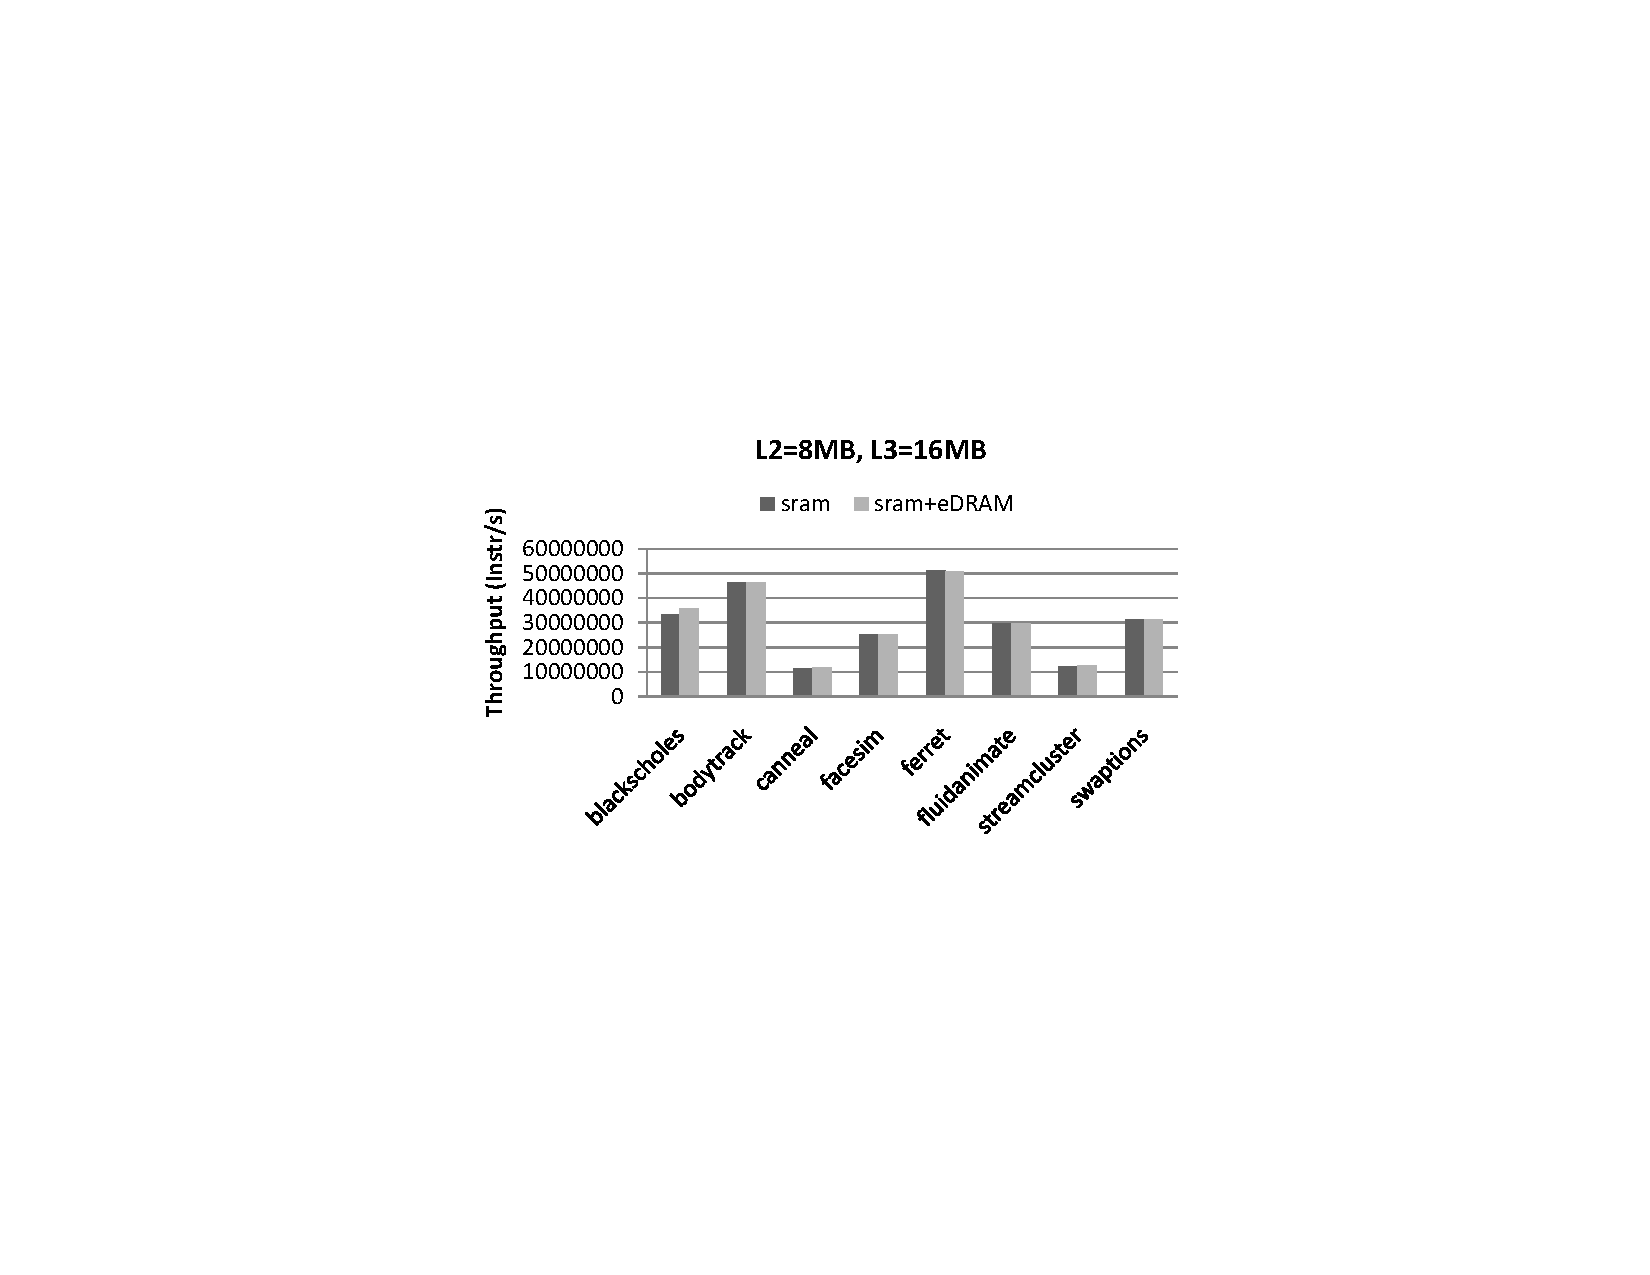
\includegraphics[width=3in]{figures/thput-l2l3-1}\hspace{0.2in}
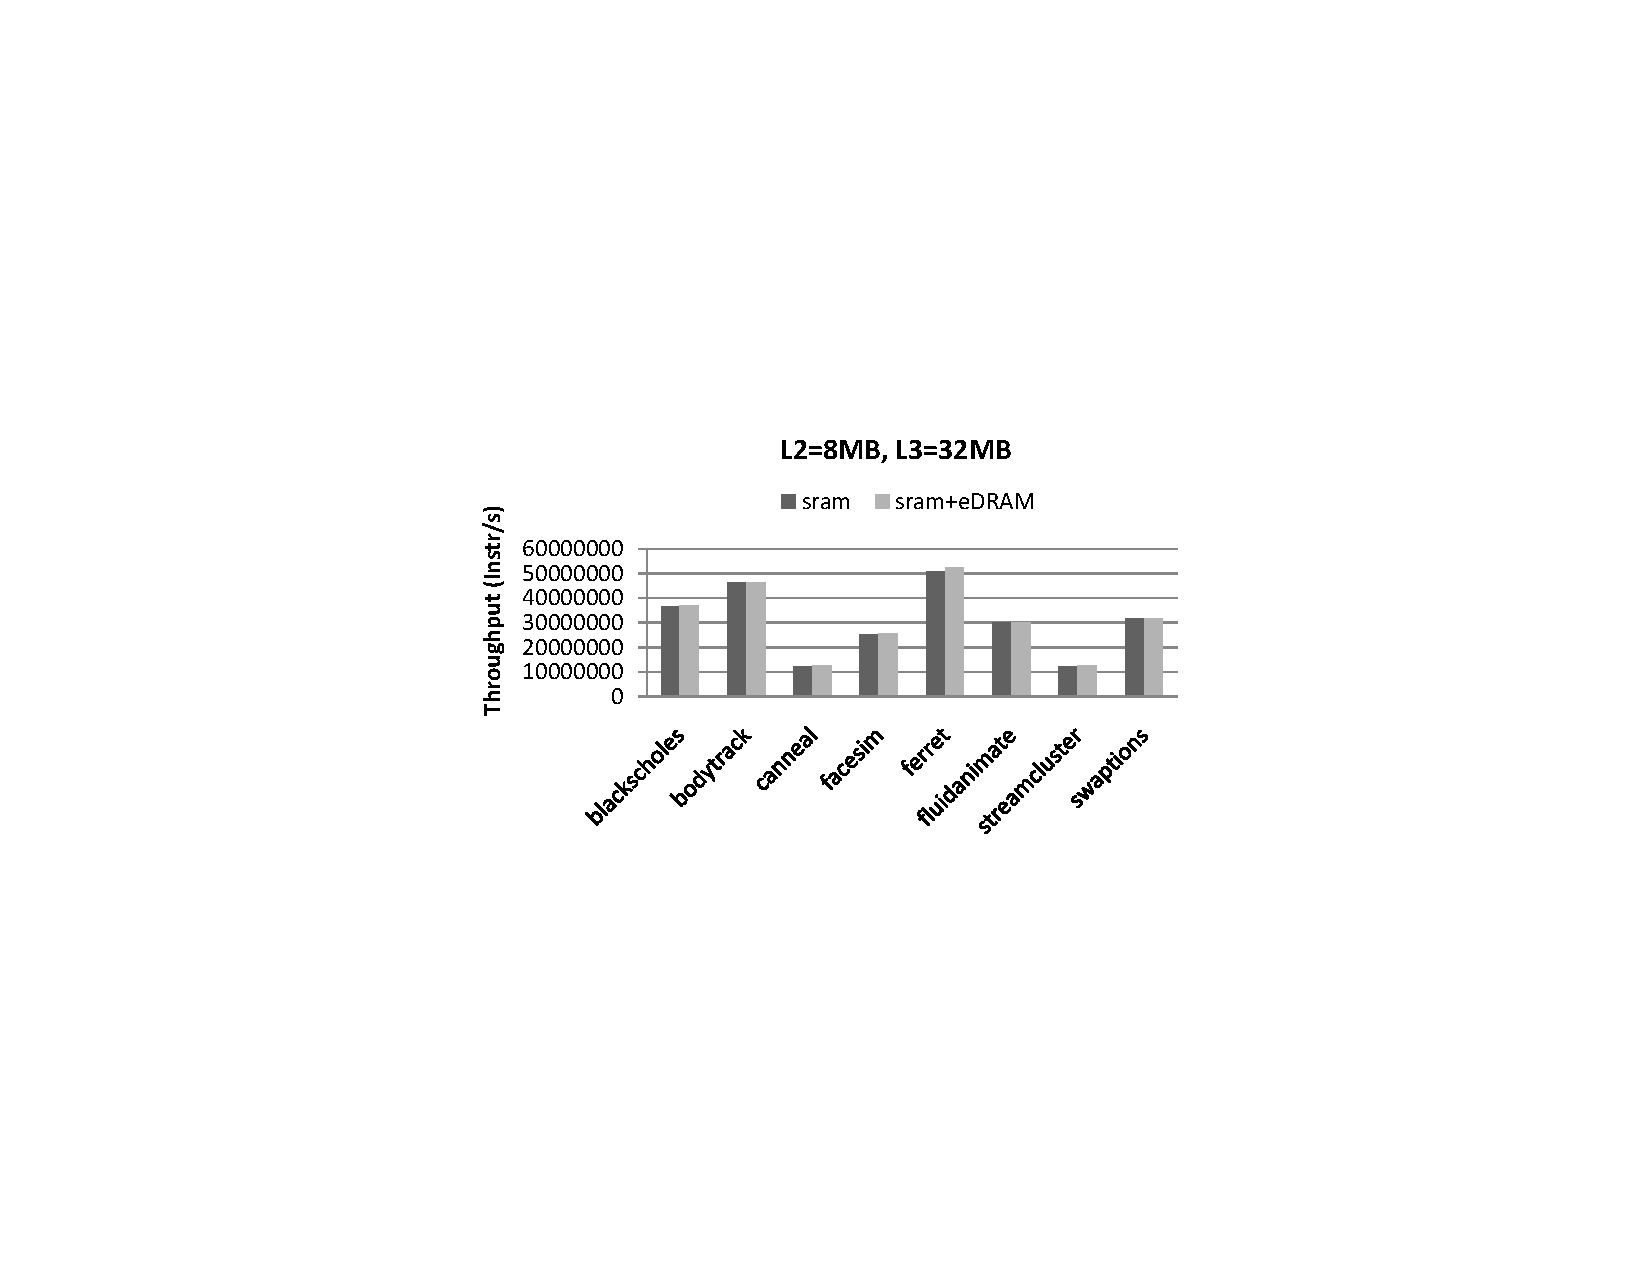
\includegraphics[width=3in]{figures/thput-l2l3-2}\\
\hspace{0.02in}
\makebox[3in][l]{\bf (a)}
\makebox[3in][l]{\bf (b)}
\caption{Performance comparison with two-level caches among various benchmarks.
  (a) The L3 cache capacity is 16MB. (b) The L3 cache capacity is 32MB.}
\label{fig:thput-l2l3}
\end{figure*}

\begin{figure*}[t]
\centering
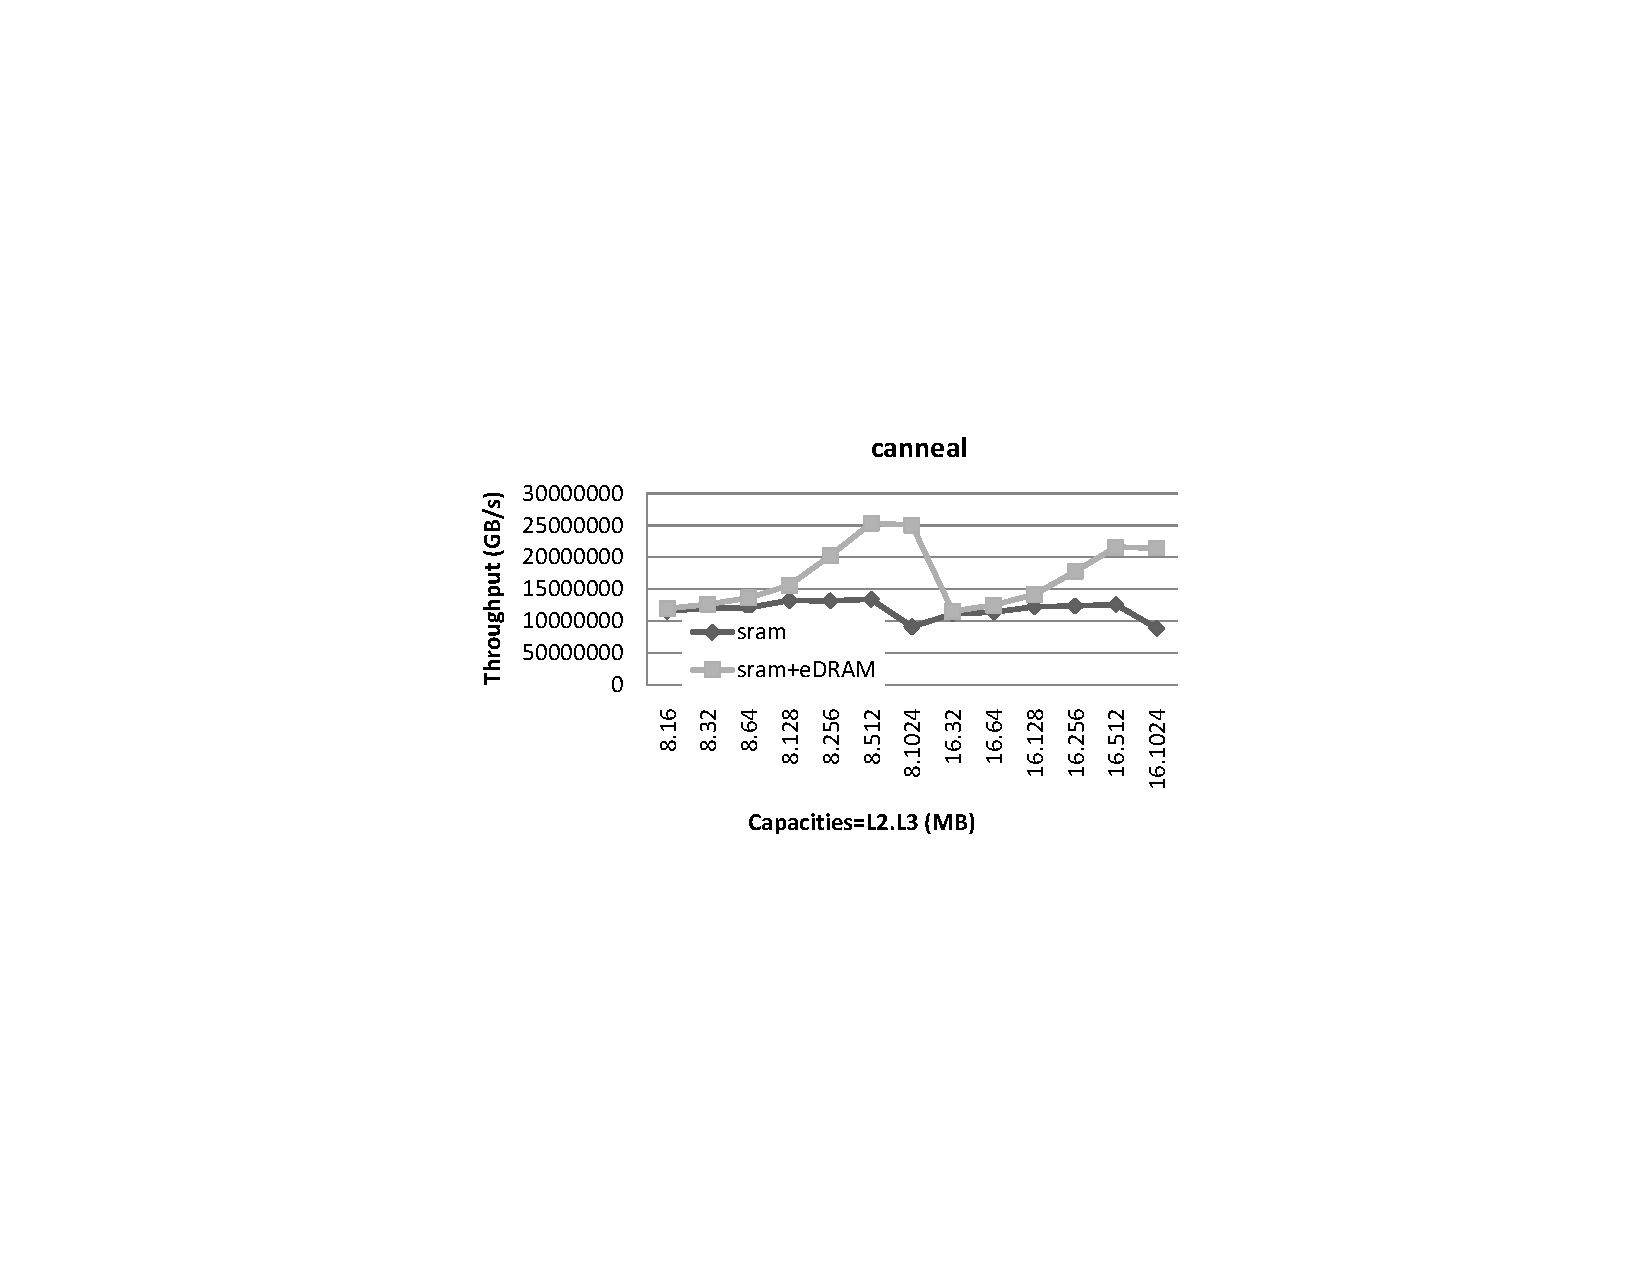
\includegraphics[width=3in]{figures/canneal-l2l3}\hspace{0.2in}
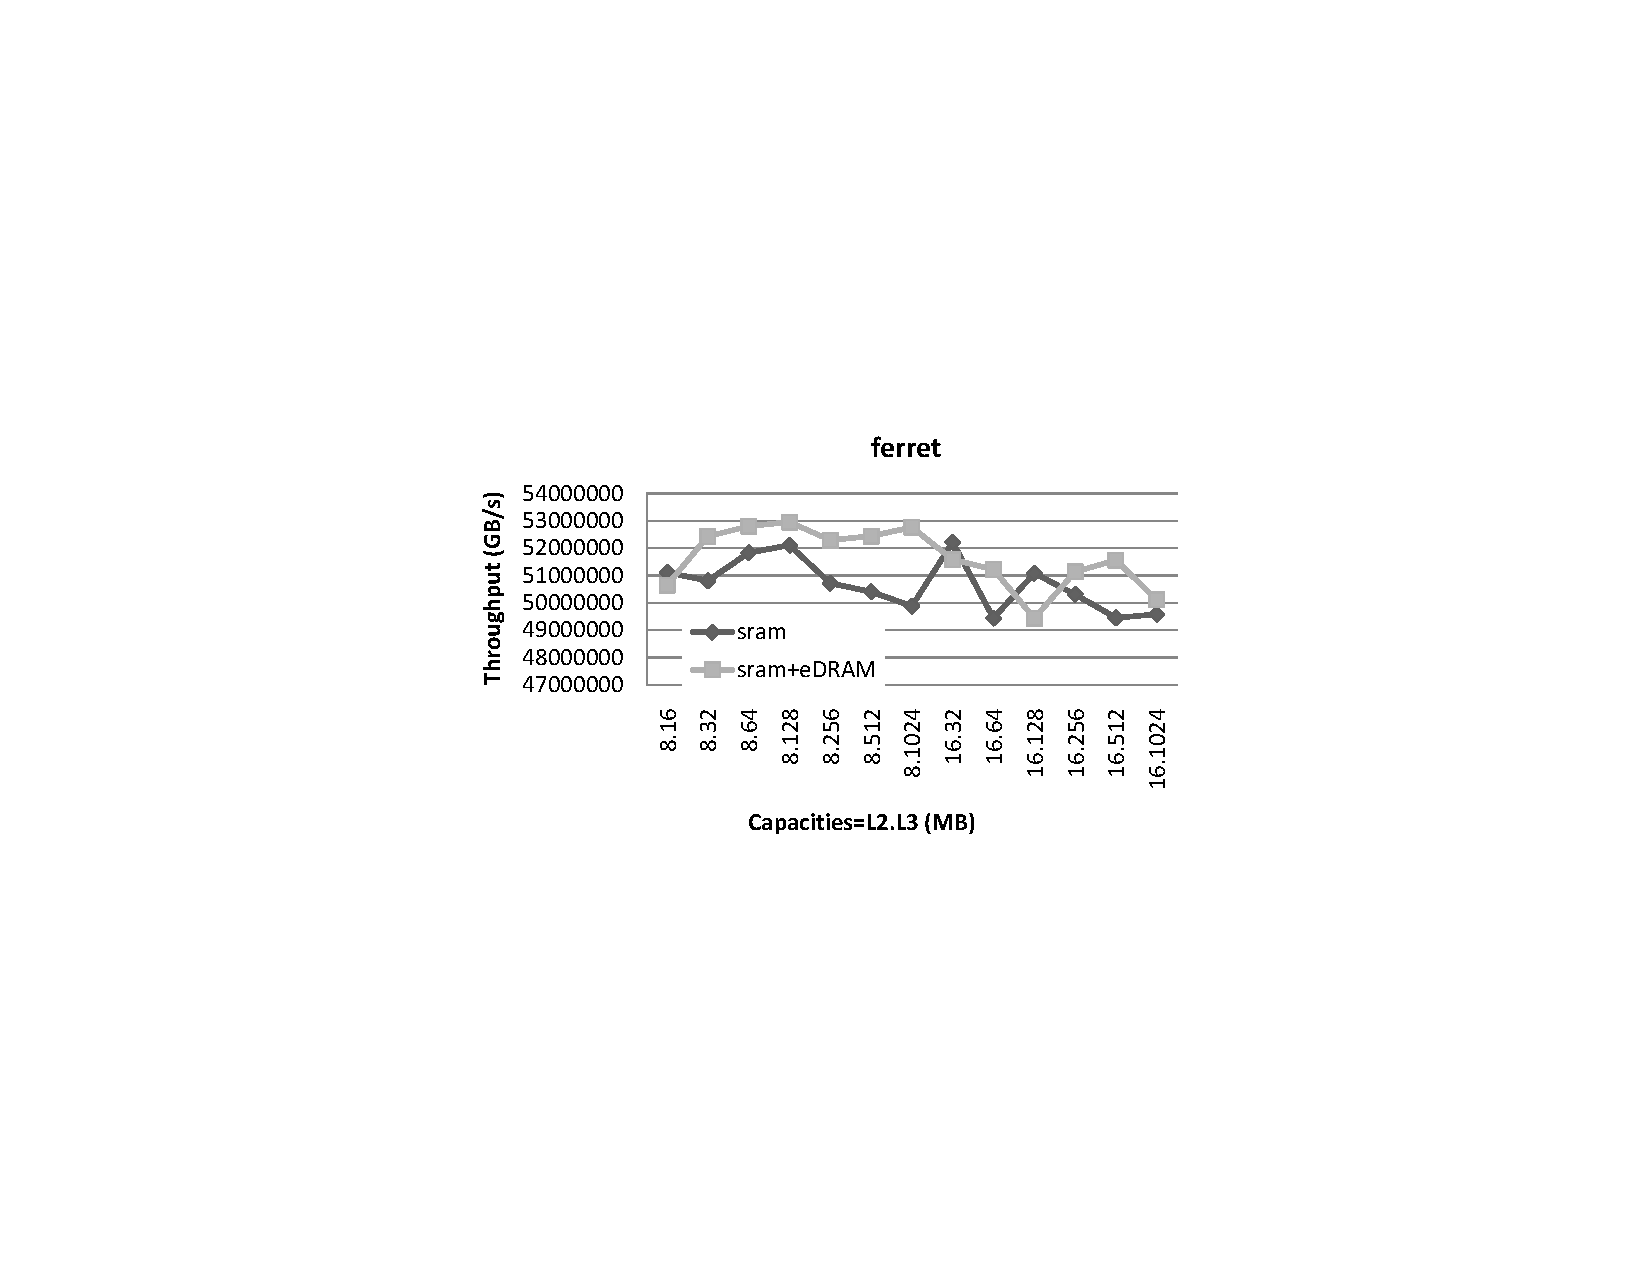
\includegraphics[width=3in]{figures/ferret-l2l3}\\
\hspace{0.02in}
\makebox[3in][l]{\bf (a)}
\makebox[3in][l]{\bf (b)}
\caption{Performance comparison with two-level caches among various cache
  capacity. (a) The canneal benchmark. (b) The ferret benchmark.}
\label{fig:benchmark-l2l3}
\end{figure*}

In the second set of experiments, we evaluate the system performance with
three-level shared caches. When evaluating hybrid cache configurations, we
consider implementing the last level cache by MRAM and RRAM memory technologies,
since the data transaction intensity is relatively low in the last level cache.
Figure~\ref{fig:thput-l2l3l4} shows the results.
Figure~\ref{fig:thput-l2l3l4}(a) illustrated that the performance more than 15\%
higher on average with a last level cache implemented by MRAM than pure SRAM
implementations. More performance improvement is obtained by increasing the last
level cache capacity, as shown in Figure~\ref{fig:thput-l2l3l4}(b).
Figure~\ref{fig:benchmark-l2l3l4} compares performance with pure SRAM and hybrid
cache implementations with different capacities. In this case, hybrid cache
implementation leads to higher performance in both benchmarks. The results of
the two sets of experiments are illustrated together in
Figure~\ref{fig:benchmark-overall}. An interesting observation is that hybrid
cache implementation shows high performance improvement with one of the
applications \emph{canneal}, whereas as little improvement with the other
\emph{ferret}. The reason is that write latency of both MRAM and RRAM is higher
than SRAM when capacity is less than 1GB. Performance of applications with large
number of writes, such as \emph{ferret} is therefore not benefit from hybrid
cache design.

\begin{figure*}[t]
\centering
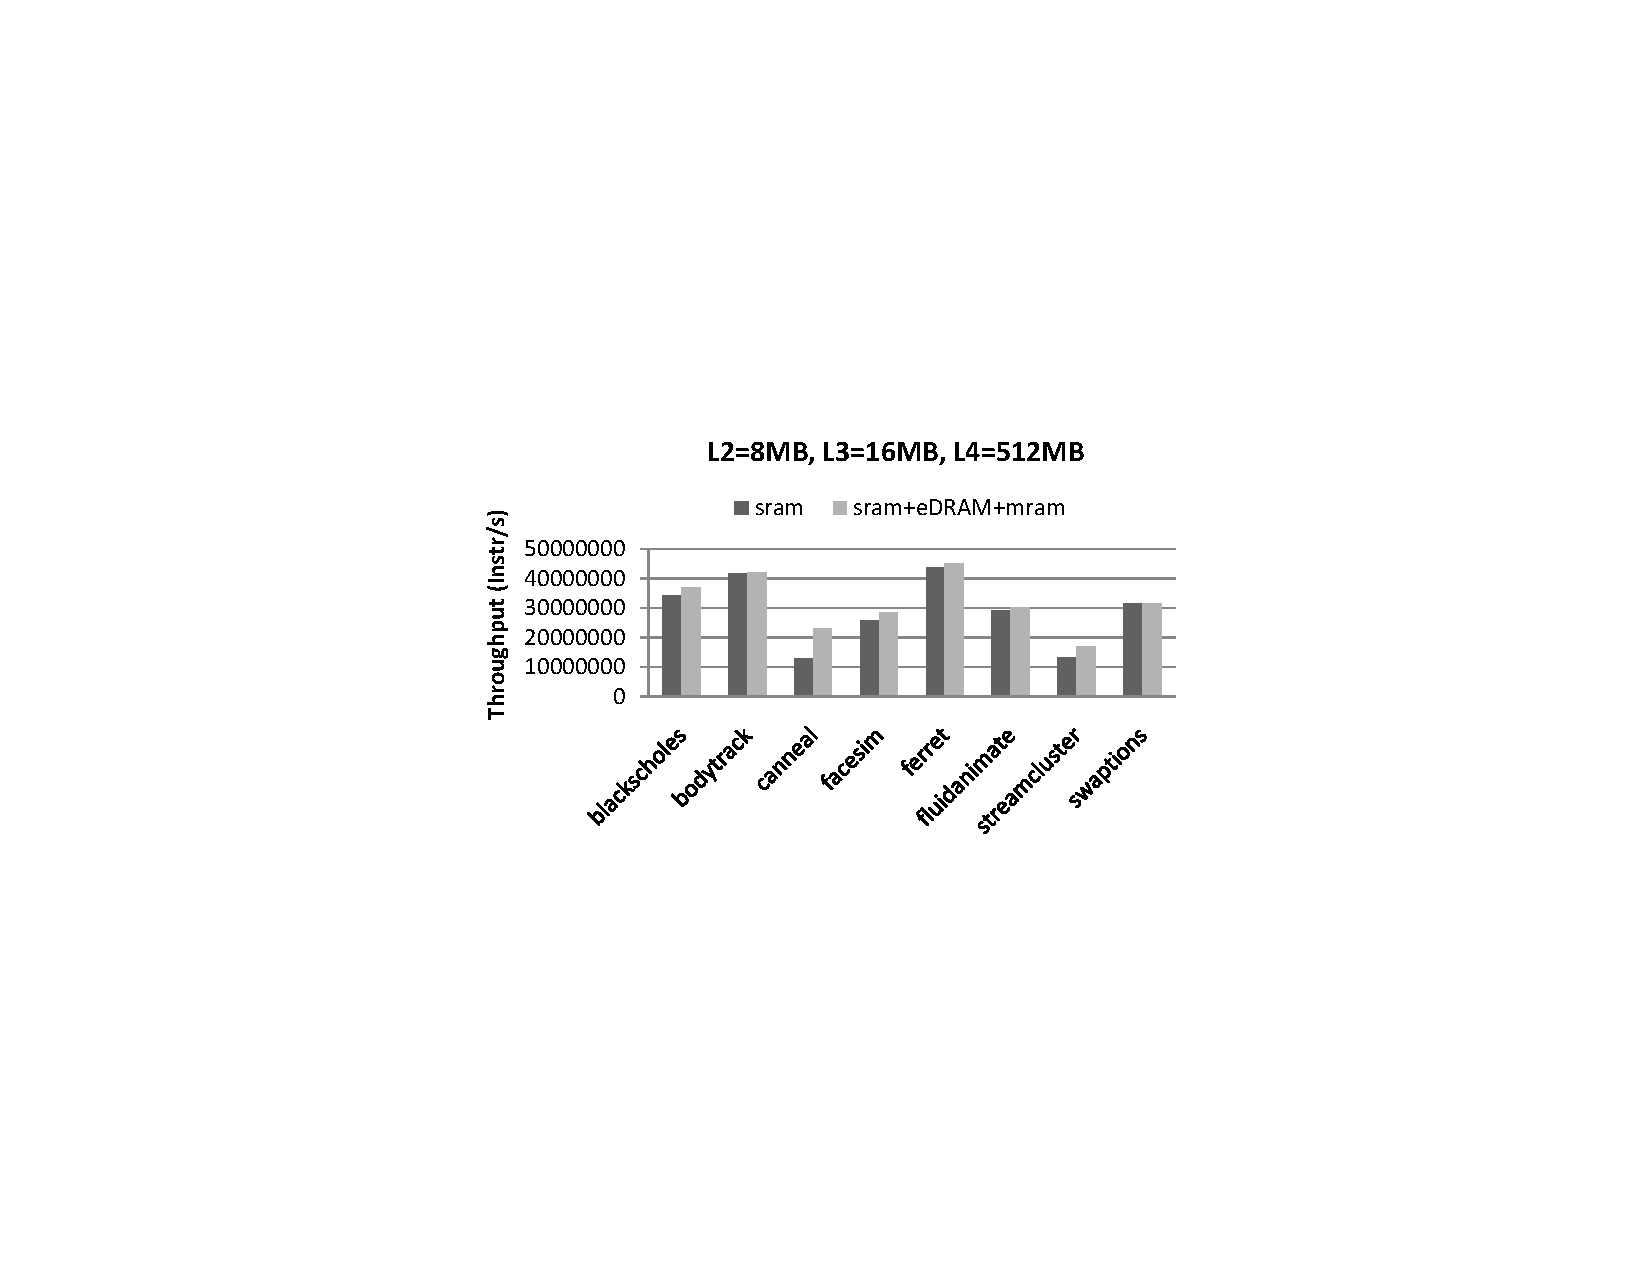
\includegraphics[width=3in]{figures/thput-l2l3l4-1}\hspace{0.2in}
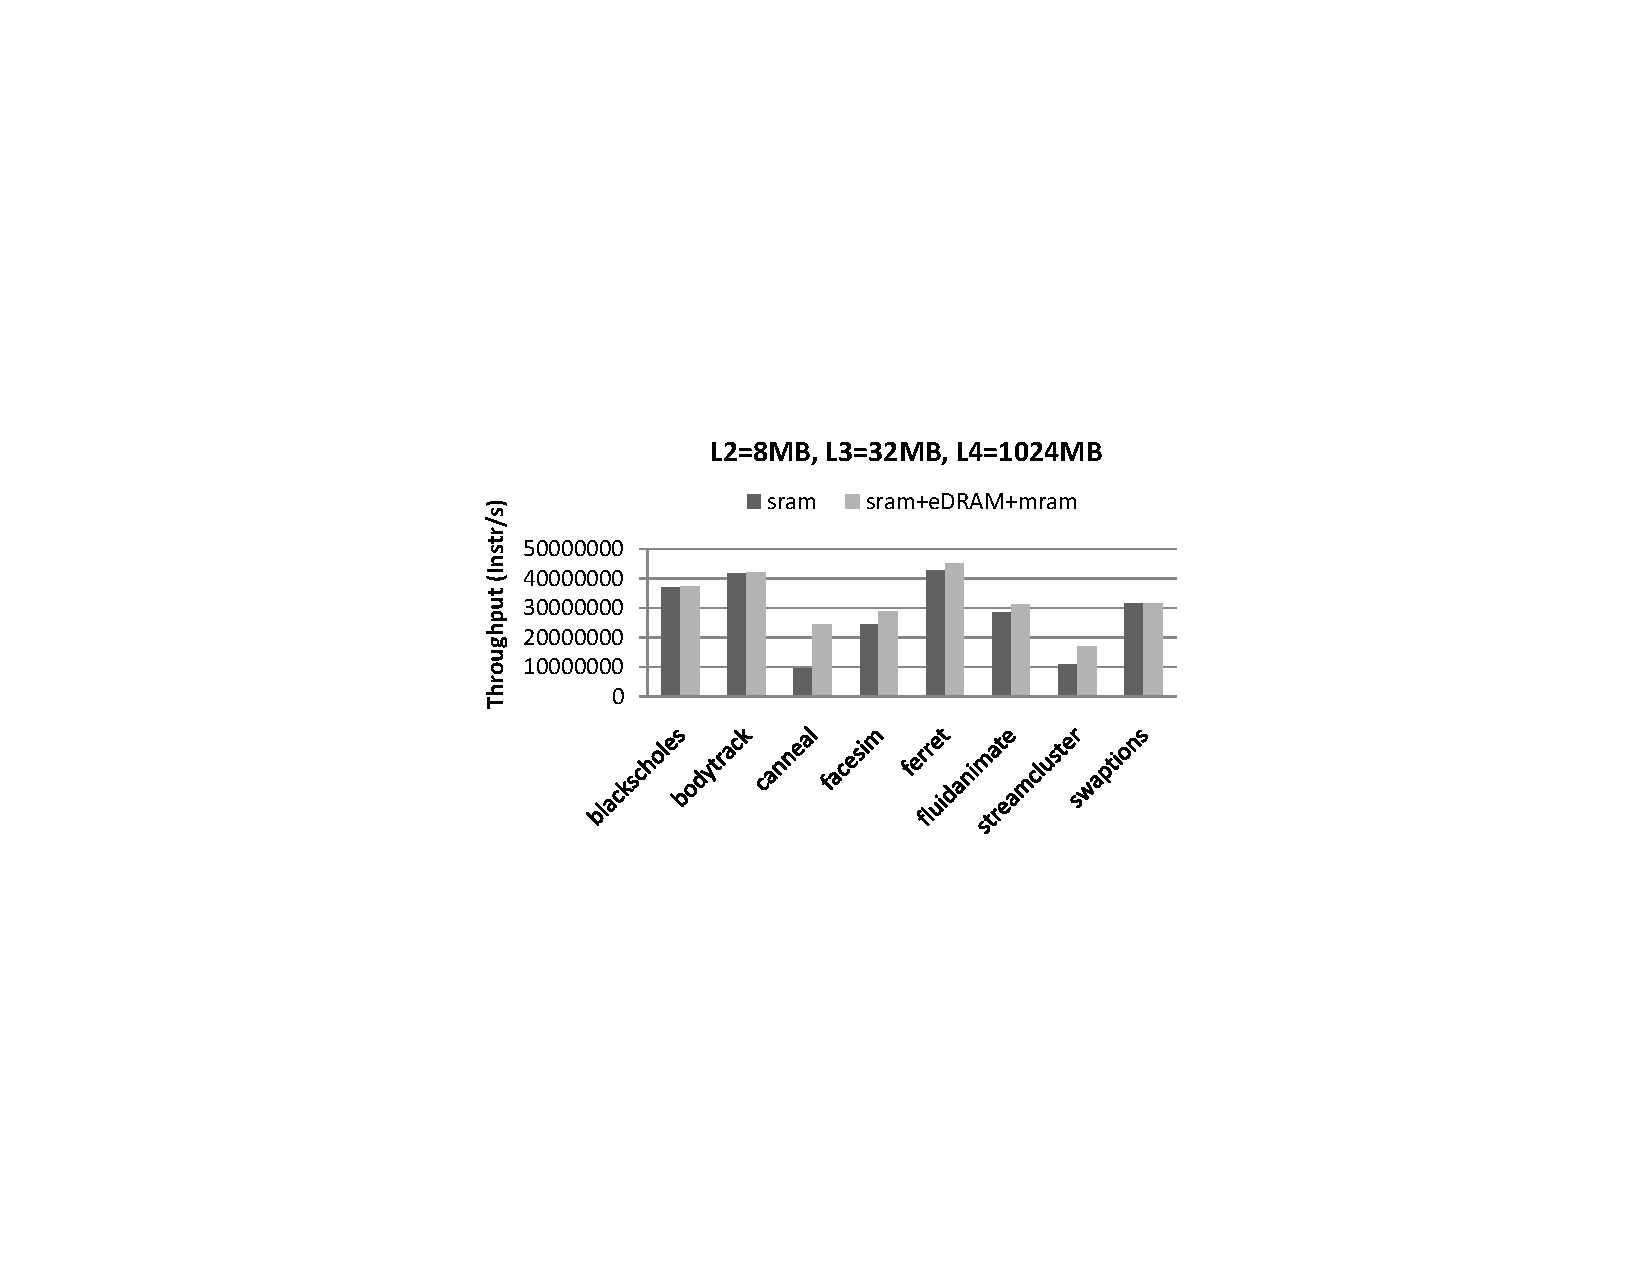
\includegraphics[width=3in]{figures/thput-l2l3l4-2}\\
\hspace{0.02in}
\makebox[3in][l]{\bf (a)}
\makebox[3in][l]{\bf (b)}

\caption{Performance comparison with three-level caches among various
  benchmarks. (a) The L3 cache capacity is 16MB, and the L4 cache capacity is
  512MB. (b) The L3 cache capacity is 32MB, and the L4 cache capacity is 1GB.}
\label{fig:thput-l2l3l4}
\end{figure*}

\begin{figure*}[t]
\centering
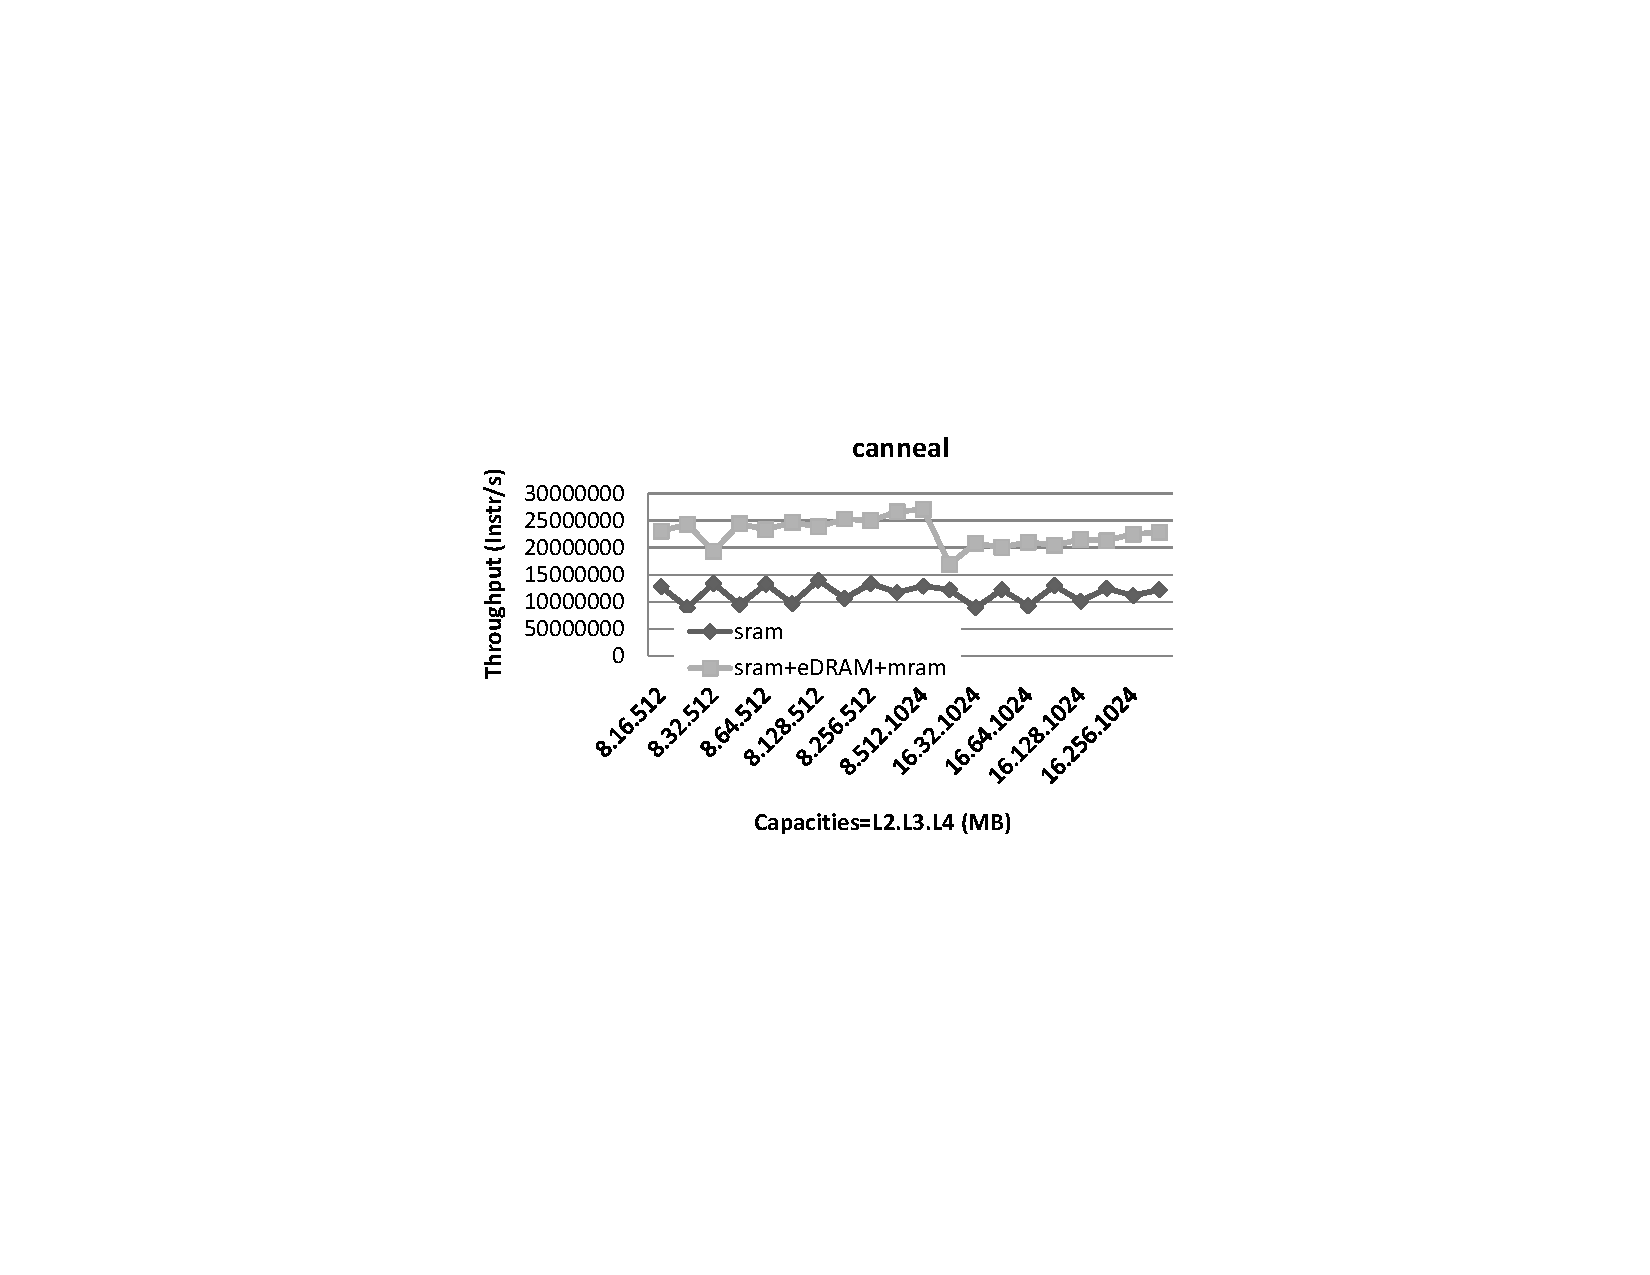
\includegraphics[width=3in]{figures/canneal-l2l3l4}\hspace{0.2in}
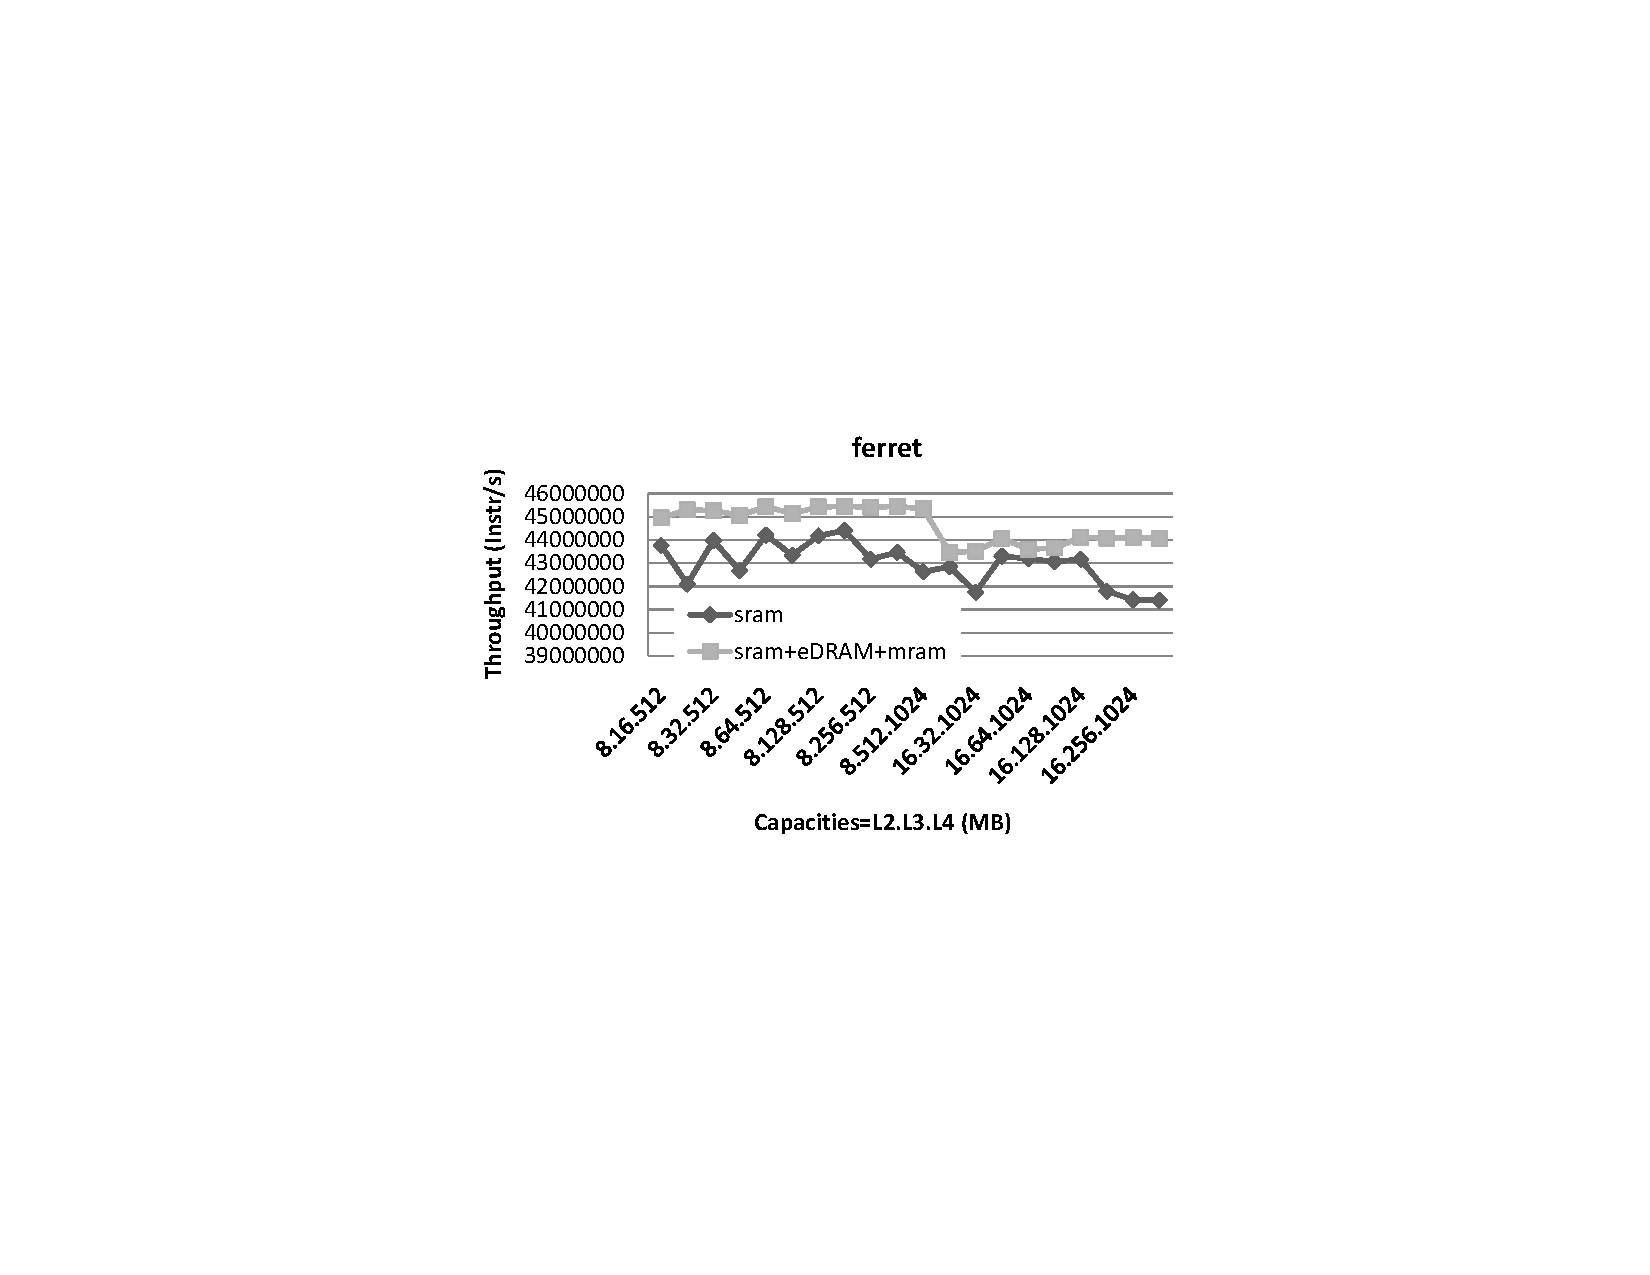
\includegraphics[width=3in]{figures/ferret-l2l3l4}\\
\hspace{0.02in}
\makebox[3in][l]{\bf (a)}
\makebox[3in][l]{\bf (b)}
\caption{Performance comparison with three-level caches among various cache
  capacity. (a) The canneal benchmark. (b) The ferret benchmark..}
\label{fig:benchmark-l2l3l4}
\end{figure*}

\begin{figure*}[t]
\centering
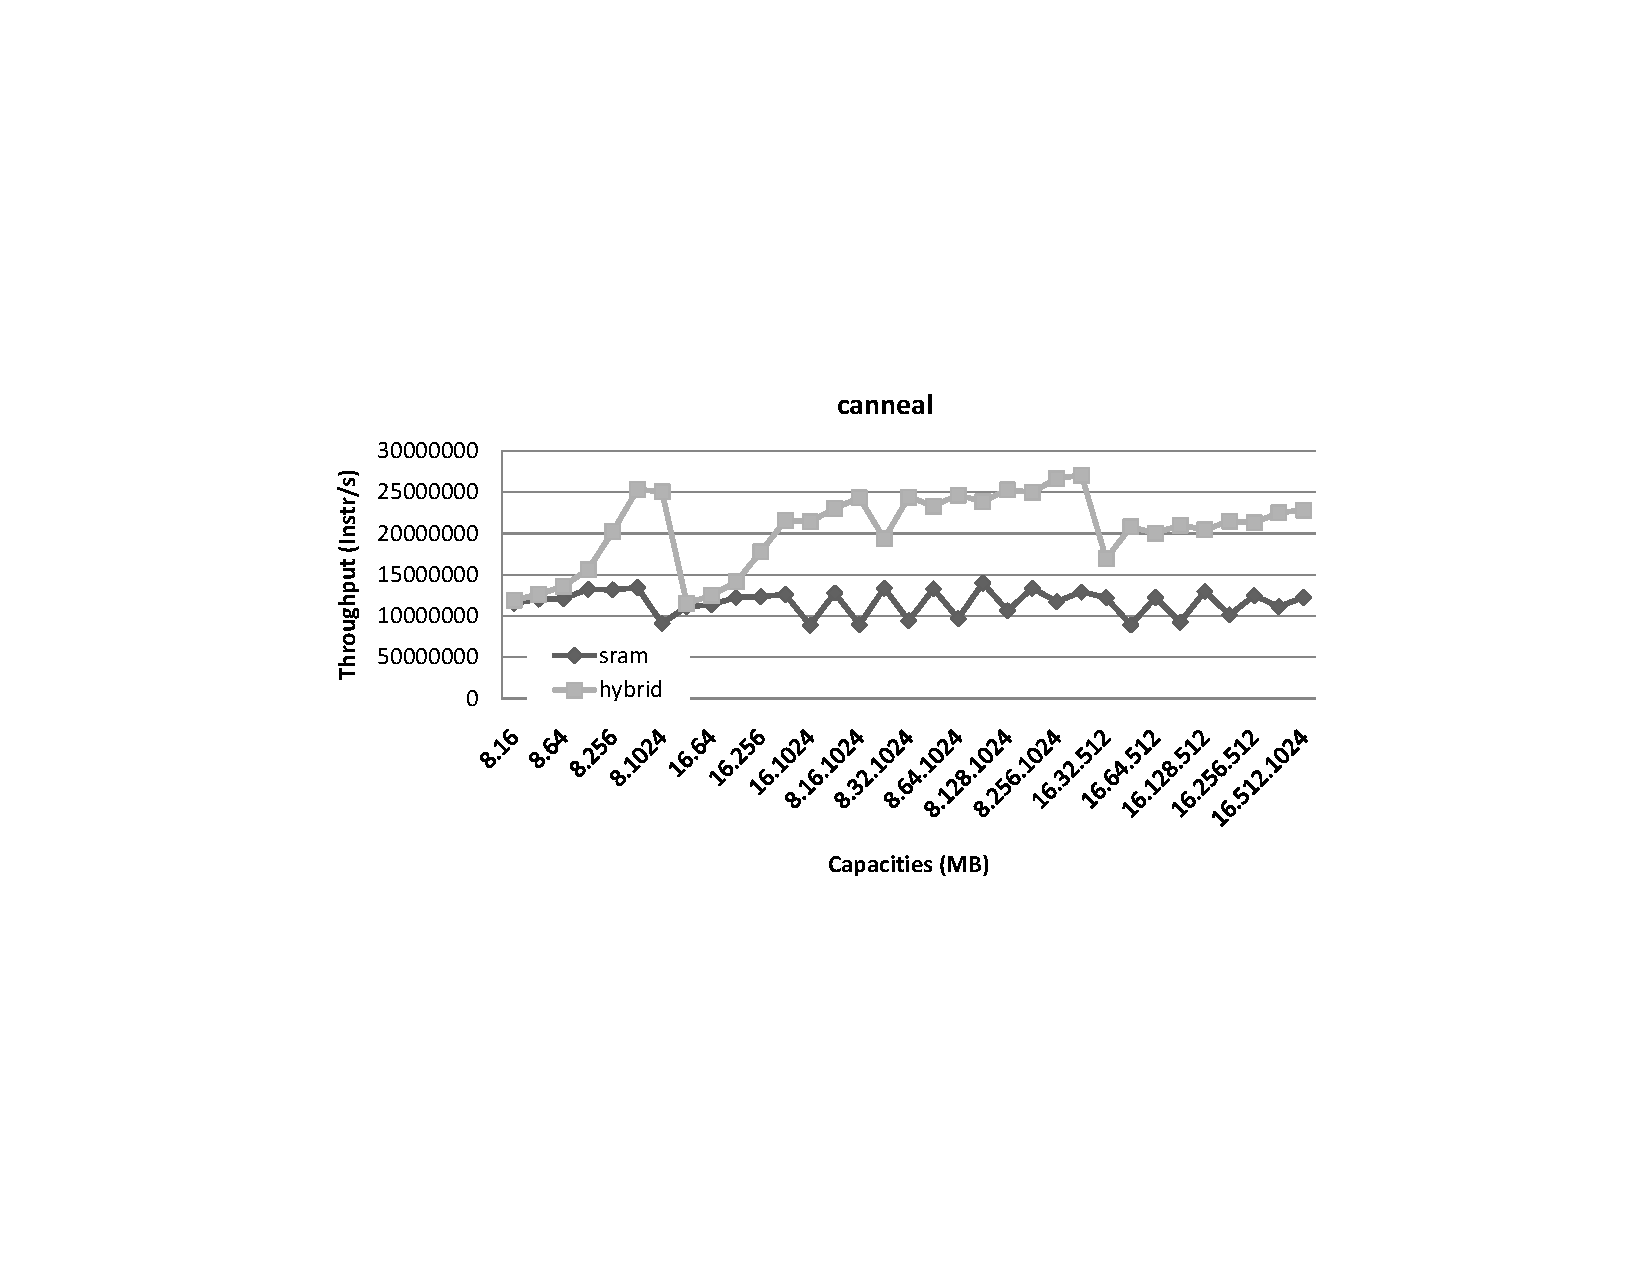
\includegraphics[width=3in]{figures/canneal}\hspace{0.2in}
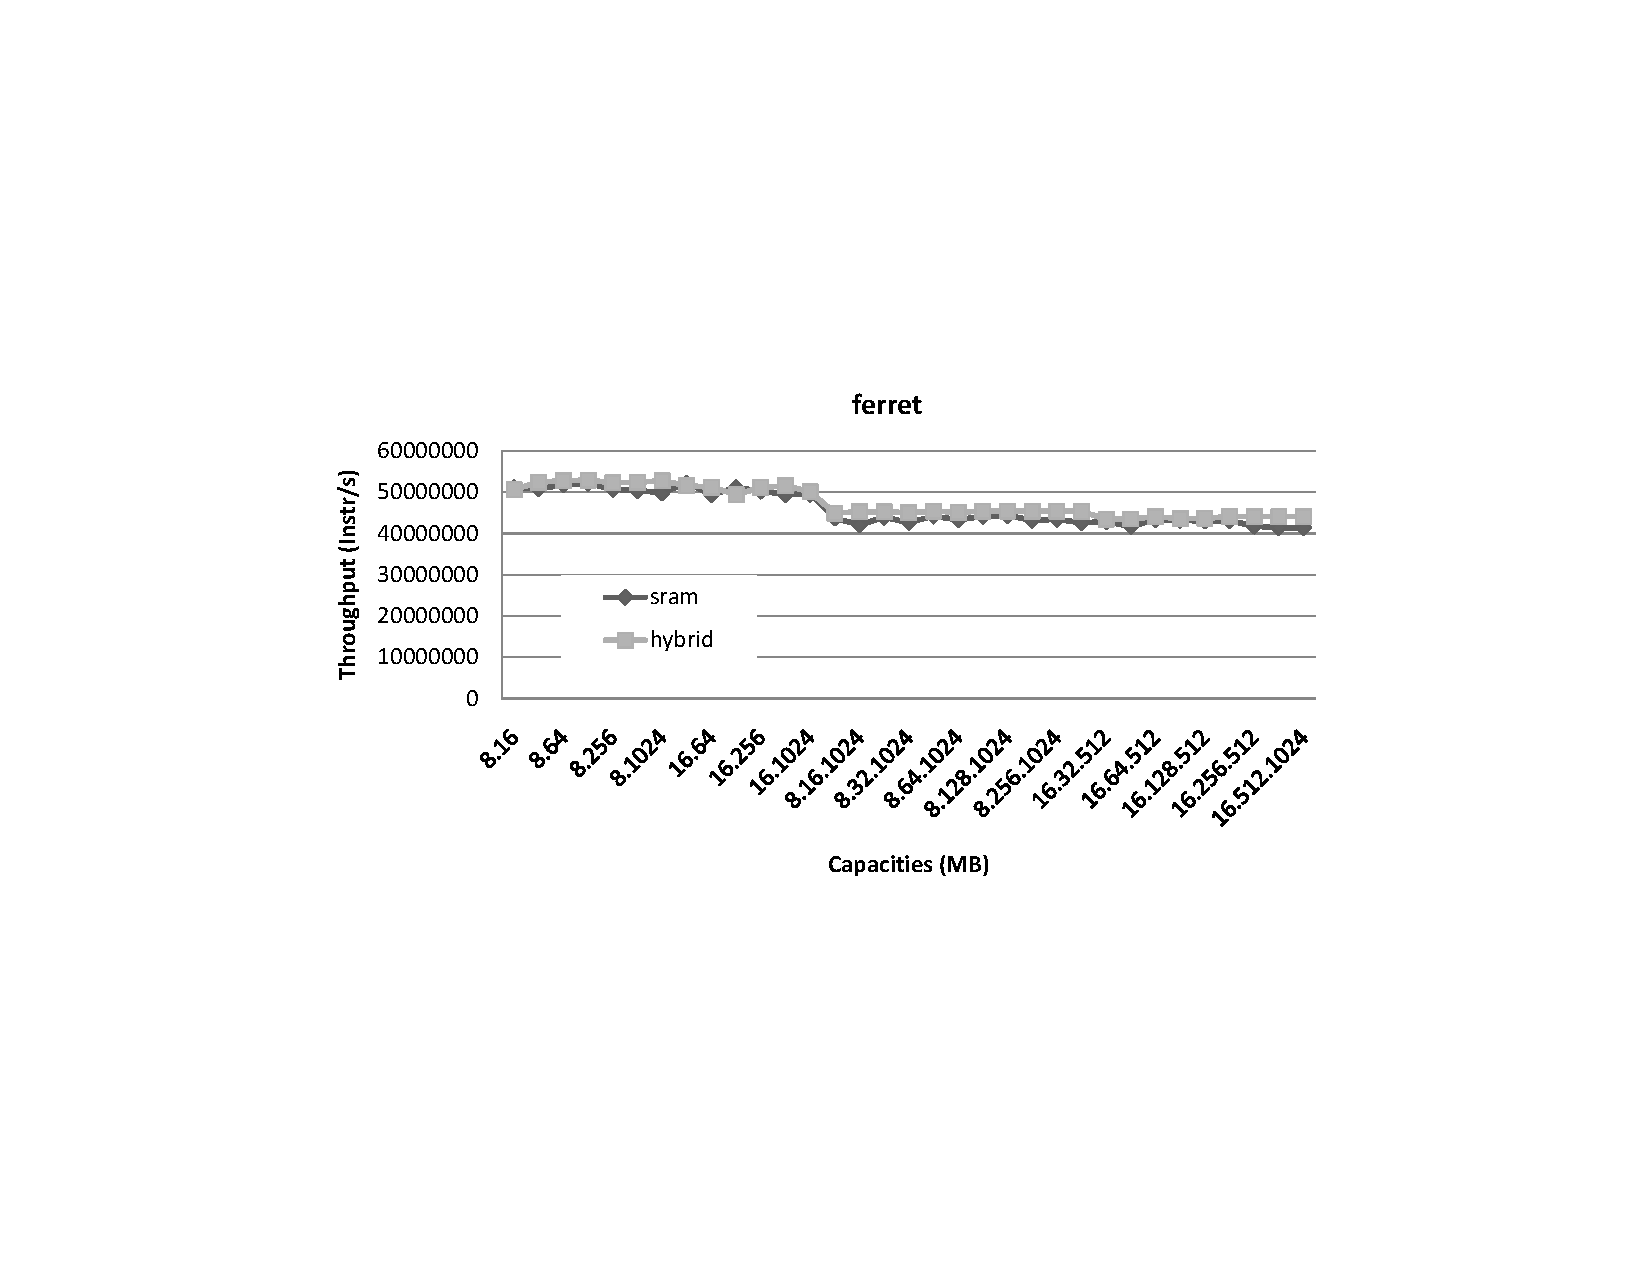
\includegraphics[width=3in]{figures/ferret}\\
\hspace{0.02in}
\makebox[3in][l]{\bf (a)}
\makebox[3in][l]{\bf (b)}

\caption{Performance comparison with both two-level and three-level caches among
  various cache capacity. (a) The canneal benchmark. (b) The ferret benchmark.}
\label{fig:benchmark-overall}
\end{figure*}

Finally, we evaluate all the possible cache hierarchy configurations with
exhaustive simulations. The optimal cache configurations of each benchmark is
shown in Table~\ref{table:results}. Since the characteristics vary among the
benchmarks, the optimal cache configurations are different among each of
benchmarks. Applications with high write intensities, such as \emph{bodytrack},
\emph{ferret}, and \emph{swaptions} tend to favor SRAM-based caches. Other
applications benefit more from hybrid cache implementation in terms of
performance.

\begin{table}[htbp!]
  \centering
  \caption{Optimal cache configurations for each benchmark.}
  \vspace{0.1in}
  \begin{tabular}{|l|c|c|c|}
    \hline
    \textbf{Benchmarks} & \textbf{L2 Configuration} & \textbf{L3 Configuration} & \textbf{L4 Configuration}\\
    \hline
    blackscholes & SRAM, 8MB & eDRAM, 32MB & RRAM, 1GB\\
    \hline
    bodytrack & SRAM, 8MB & eDRAM, 128MB & -\\
    \hline
    canneal & SRAM, 8MB & eDRAM, 512MB & MRAM, 1GB\\
    \hline
    facesim & SRAM, 8MB & eDRAM, 32MB & MRAM, 1GB\\
    \hline
    ferret & SRAM, 8MB & eDRAM, 32MB & -\\
    \hline
    fluidanimate & SRAM, 8MB & eDRAM, 1GB & -\\
    \hline
    streamcluster & SRAM, 16MB & eDRAM, 128MB & MRAM, 512MB\\
    \hline
    swaptions & SRAM, 8MB & SRAM, 32MB & SRAM, 1GB\\
    \hline
  \end{tabular}
  \label{table:results}
\end{table}

\section{Conclusion and Future Work}
In this project, we explore performance and energy characteristics of various
emerging memory technolgies. Based on our exploration, we evaluate the shared
cache hierarchy design of CMPs optimized for performance by filling the off-chip
memory bandwidth gap. According to our evaluation, SRAM-based caches leads to
reasonable performance with write-intensive applications. Hybrid cache design
help with performance with other types of benchmarks.

Furthermore, a variety of continuing studies is remained to be explored related
to bandwidth-aware memory hierarchy design. First of all, we only examine cache
hierarchy design currently. It is necessary to extend our exploration to the
overall memory hierarchy design. On the other hand, we do not consider energy
efficiency in this project. We would like to put some power constraints to the
memory hierarchy, and examine the energy efficiency of various memory hierarchy
configurations.

% \bibliographystyle{IEEEtran}
\bibliographystyle{latex8}
\bibliography{./bib/ref,./bib/reram,./bib/cacti}

\end{large}

\end{document}
